\documentclass[a4wide]{article}
\usepackage{a4wide}
\usepackage{pgf}
\usepackage[latin1]{inputenc}
\usepackage{listings}
\usepackage{hyperref}
\usepackage{subfigure} 
\usepackage{tikz}
\usepackage{algorithm}
\usepackage{algpseudocode}
\usepackage{caption}
\usepackage{rotating}
\usepackage{amsmath,amsthm}
\usepackage{amssymb}
\usepackage{tikz}
\usepackage{url}
\usepackage{comment}
\usepackage{enumitem}
\usetikzlibrary{arrows}
\usepackage[autostyle]{csquotes}

\newtheorem*{definition}{Definition}

\definecolor{cgreen}{rgb}{0.05, 0.5, 0.06}

\tikzset{
  treenode/.style = {align=center, inner sep=0pt, text centered,
    font=\sffamily},
  arn/.style = {treenode, circle, black, font=\sffamily\bfseries, draw=black,
    fill=white, text width=1.5em},
}

\lstset{
numbers=left, 
numberstyle=\small, 
numbersep=8pt, 
frame = single, 
language=C++, 
framexleftmargin=14pt}

%\textwidth = 390pt
%\textheight = 900pt
\parindent 0mm


\begin{document}

\title{Algorithms for tree decompositions -- an implementation\\
\small{version 0.6.0}}
\author{Lukas Larisch}

\date{\today}
\maketitle


Funded by the German Research Council, Project GalA, AD 411/1-1 \\

\vspace*{0.6cm}

We implemented various algorithms for computing tree decompositions of graphs. \\
Our implementation includes \\

\begin{itemize}
\item A preprocessing with running time $O(n^3)$ \cite{B_tc3, A_P_rec}, consisting in
the repeated application of reduction rules, which in case the
input graph G has tree-width at most 3 allow us to determine it's tree-width exactly and, in addition, compute the corresponding tree decomposition. If the tree-width is larger, the reduction rules return a possibly smaller instance of the same tree-width as the original graph,

\item Several algorithms, that compute a lower bound on the tree width of a given graph \cite{B_lb_db, CC_lb_nw, B_tc2, L_lb_mcs},

\item An algorithm based on the cops and robber game \cite{ST_minmax}, which
for a given graph G and an integer k decides whether $tw(G)\leq k$,
and if this is the case, returns a tree decomposition of width at most
k. The algorithm runs in time $n^{O(k)}$. \\
We run the algorithm for k=1,2,3,... to determine the tree-width exactly,

\item Another algorithm based on the cops and robber game, which for a given graph G and an integer k decides whether $tw(G)\leq k$,
and if this is the case, returns a tree decomposition of width at most
k. The algorithm runs in time $O(n!)$. \\
Again we run it for k=1,2,3,... to determine the tree-width exactly. This algorithm may be faster than the above mentioned one,

\item Various heuristics of elimination orderings, including the minDegree and minFill-heuristics \cite{B_tc1},  

\item The separator algorithm \cite{R_sep}, which for a given graph G and
an integer k correctly returns $'tw(G)>k'$ if this is the case, and
if $tw(G) \leq k$, then the algorithm computes a tree decomposition
of $G$ of width at most $4 \cdot tw(G)$, which allows us to approximates the tree-width up to a factor of 4. The algorithm runs in time $2^{O(k)} \cdot poly(n)$, where $n$ is the number of vertices of the input graph,

\item Postprocessing, containing the MinimumSeperatingVertexSets-heuristic \cite{B_tc3, Koster_thesis} and the minimalChordal algorithm of Heggernes \cite{BHS_md}, which may reduce the width of a given tree decomposition.

\item Algorithms for solving hard problems based on tree decompositions, including Clique, Vertex Cover, Independent Set, Dominating Set and Colorability.

\end{itemize}

\newpage

\tableofcontents

\section{Overview on all implemented algorithms}

All algorithms have been implemented in C++ using the Boost Graph Library \cite{boost}. Following tables give an overview over all implemented algorithms:\\

\begin{table}[h!]
\small
\begin{tabular}{l|l|l|l}
preprocessing & exact algorithms & approximate algorithms & postprocessing \\
\hline
\hline
reduction rules for tw $\leq$ 1 & greedy cops \& robbers & seperator algorithm & MSVS\\
reduction rules for tw $\leq$ 2 & dynamic cops \& robbers & minDegree heuristic & triang. minimiz.\\
reduction rules for tw $\leq$ 3  & & minFill heuristic \\
some red. rules for tw $\leq$ 4 & & \\
red. rule for almost simplicial vert. & & \\
\hline
\end{tabular}
\normalsize
\caption{Implementations of preprocessing, exact algorithms, approximate algorithms and postprocessing.}
\end{table}

\vspace*{5mm}

\begin{table}[h!]
\begin{tabular}{|l|l|l|}
\hline
degree based & improved graphs & miscellaneous \\
\hline
\hline
delta & LBN-deltaD & MCS \\
delta2 & LBN-deltaC & MCSC-min-deg \\
gamma & LBNC-deltaD & MCSC-last-mcs \\
deltaD & LBNC-deltaC & MCSC-max-mcs \\
delta2D & LBP-deltaD &\\
gammaD-left & LBP-deltaC &\\
gammaD-right & LBNP-deltaD &\\
gammaD-min-e & LBNP-deltaC &\\
deltaC-min-d &&\\
deltaC-max-d &&\\
deltaC-least-c &&\\
\hline
\end{tabular}
\caption{Tree-width lower bound algorithms}
\end{table}

Implementation of algorithms for solving hard problems based on tree decompositions for the following problems.

\begin{itemize}
\item max-Clique
\item min-Vertex Cover
\item max-Independent Set
\item min-Dominating Set
\item min-Colorability
\end{itemize}

Furthermore some useful algorithms for tree decompositions in general have been implemented.

\begin{itemize}
\item is\_valid\_decomp: tests whether a tree decomposition is valid with respect to a graph 

\item treedec\_to\_elimination\_ordering: transforms a tree decomposition to an elimination ordering

\item elimination\_ordering\_to\_treedec: transforms an elimination ordering to a tree decomposition

\item treedecomposition\_to\_branchdecomposition: converts a tree decomposition to a branch decomposition 

\item branchdecomposition\_to\_treedecomposition: converts a branch decomposition to a tree decomposition 

\item make\_small: makes a tree decomposition small

\item nicify\_treedecomposition: makes a tree decomposition a nice tree decomposition
\end{itemize}

\section{Testset}

The implementation has been tested on 1817 control flow graphs and all graphs contained in the DIMACS-challenge for graph-coloring \cite{dimacs} and some "named graphs", which we call zoo here. The control-flow graphs were obtained from the iCode in the sdcc compiler \cite{sdcc} by compiling, the sdcc standard C library from the 3.5.0 sdcc release, a C version of the floating-point benchmark Whetstone \cite{whetstone}, an ISO C version of version 2 of the integer benchmark Dhrystone \cite{dhrystone,dhrystone2} and the benchmark Coremark \cite{coremark}, version 2.5 of the operating system Contiki \cite{contiki}and the operating system FUZIX (from the git repository as of 2015-01-08). \\

Control flow graphs of the programming language C without use of gotos have bounded treewidth by 7 \cite{thorup, C-tree}.
The graphs from DIMACS-challenge for graph-coloring are extremly hard to color and hence have huge treewidth. \\ 

All measure of time have been made without reading/writing the graphs. \\

\section{Input format}

Input graphs have to be boost graphs (i.e. have to provide the boost graph interface). They need to be undirected in most cases. Treedecompositions are representated by undirected graphs with sets attached to nodes.

\begin{lstlisting}[mathescape]
#include<tdlib/graph.hpp>

typedef boost::adjacency_list<
   boost::setS,
   boost::vecS,
   boost::undirectedS
  > graph_t;
typedef boost::adjacency_list<
   boost::vecS,
   boost::vecS,
   boost::undirectedS,
   treedec::bag_t
  > tree_dec_t;
\end{lstlisting}

\newpage

\section{Preprocessing}

In the following, assume that the input graph G containes an induced subgraph H as shown in the figures below, where red-colored vertices have the same degree in G as in the figures. The configuration of fixed-degree vertices in the following rules makes it possible to check the applicability of a rule for a fixed vertex x' $\in$ V(G) in constant time. e.g. where we assume x' will be mapped to the given vertex x $\in$ H. Then, if we demand $d_{G}(x') = 3$ and, in addition, at least two of three neighbours y', z' of x' must have fixed degree, there are at most 3 choices of y' and z', for which we have to test remaining properties of \enquote{wider surroundings} (e.g. the 2-neighbourhood) of x'. If at least one property does not hold for all possible choices of neighbours of x', we know, that there does not exist a function $\pi: V(H) \rightarrow V(G)$, $\pi(x) = x'$, such that $d_{G}(\pi(x)) = d_{H}(x)$ and $G[\pi(V(H))] \cong H$. In this manner, we can successivly test, whether the neighbourhood of x' in G looks like the neighbourshood of x in H, where H is the graph, defined by the figures. If this procedure succeeds, we know, that a specific rule is applicable at x' in G and we will eliminate x, resulting in $N_{G}[x']$ as a bag of a tree decomposition of G.

\subsection{Rules}

Various rules to preprocess a given graph G, such that the reduced graph may be a smaller instance according to compute a tree decomposition or the treewidth have been implemented. A graph G can be reduced to the empty graph by
\begin{itemize}
\item Islet $\Leftrightarrow$ tw(G) = 0
\item Islet and Twig $\Leftrightarrow$ tw(G) $\leq$ 1
\item Islet, Twig and Series $\Leftrightarrow$ tw(G) $\leq$ 2
\item Islet, Twig, Series, Triangle, Buddy and Cube $\Leftrightarrow$ tw(G) $\leq$ 3
\end{itemize}

\vspace{2mm}

If a graph is not fully reducable by Islet, Twig, Series, Triangle, Buddy and Cube, we know that its treewith is greater than 3, such that the preprocessing rules provide a small lower bound according to treewidth. A maximum sized bag produced by the rules Simplicial or AlmostSimplicial also gives a lower bound. \\

Both an algorithm for each rule, that applies the rule to a graph if possible and creates the corresponding bag, and the graph fitting to the rule will be given in the following.
red-colored vertices have to be connected as shown. green-colored vertices possibly have further edges.\\

\begin{minipage}{0.5\textwidth}
\underline{\textbf{Islet}} \cite{B_tc3, E_B_safe} \\ \\
Iterate through all vertices v $\in$ G. \\
If $d_{G}(v) == 0$:  \\
Create a bag \{v\} and remove v. \\
\end{minipage}
\hspace{3.0cm}
\begin{minipage}{0.5\textwidth}

\begin{tikzpicture}[->,>=stealth',shorten >=1pt,auto,node distance=3cm,
  thick,main node/.style={circle,fill=red,draw,font=\sffamily\Large\bfseries}]
  \node[main node] (1) {v};
\end{tikzpicture} \\
\end{minipage}

\vspace*{0.5cm}

\begin{minipage}{0.5\textwidth}
\underline{\textbf{Twig}} \cite{B_tc3, E_B_safe} \\ \\
Iterate through all vertices v $\in$ G. \\
If $d_{G}(v) == 1$: \\ 
Let w be the neighbour of v. \\
Create a bag \{v, w\} and remove v. \\
\end{minipage}
\hspace{3.0cm}
\begin{minipage}{0.5\textwidth}
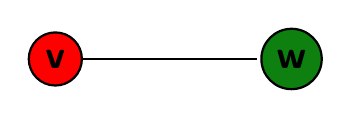
\begin{tikzpicture}[-,>=stealth',shorten >=1pt,auto,node distance=3cm,
  thick,main node/.style={circle,fill=red,draw,font=\sffamily\Large\bfseries},
        others node/.style={circle,fill=cgreen,draw,font=\sffamily\Large\bfseries}]
  \node[main node] (1) {v};
  \node[others node] (2) [right of=1] {w};
  
  \path[every node/.style={font=\sffamily\small}]
    (1) edge (2);
\end{tikzpicture} \\
\end{minipage}

\vspace*{0.5cm}

\begin{minipage}{0.5\textwidth}
\underline{\textbf{Series}} \cite{B_tc3, E_B_safe} \\ \\
Iterate through all vertices v $\in$ G. \\
If $d_{G}(v) == 2$: \\
Let w and u be the neighbours of v. \\
Remove v, add an edge \{w, u\} to G and create a bag \{v, w, u\}. \\
\end{minipage}
\hspace{2.0cm}
\begin{minipage}{0.5\textwidth}
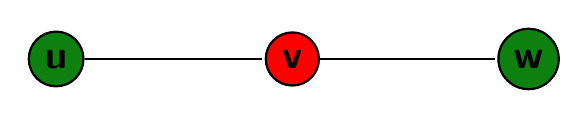
\begin{tikzpicture}[-,>=stealth',shorten >=1pt,auto,node distance=3cm,
  thick,main node/.style={circle,fill=red,draw,font=\sffamily\Large\bfseries},
        others node/.style={circle,fill=cgreen,draw,font=\sffamily\Large\bfseries}]
  \node[main node] (1) {v};
  \node[others node] (2) [right of=1] {w};
  \node[others node] (3) [left of=1] {u};
  
  \path[every node/.style={font=\sffamily\small}]
    (1) edge (2)
    (3) edge (1);
\end{tikzpicture} \\
\end{minipage}

\vspace*{0.5cm}

\begin{minipage}{0.5\textwidth}
\underline{\textbf{Triangle}} \cite{A_P_rec} \\ \\
Iterate through all vertices v $\in$ G. \\
If $d_{G}(v) == 3$: \\
Let x, y and z the neighbours of v. If there is at least one edge \{x, y\}, \{x, z\} or \{y, z\}, remove v, create a bag \{v, x, y, z\} and make x, y and z a clique. \\
\end{minipage}
\hspace{2.0cm}
\begin{minipage}{0.5\textwidth}
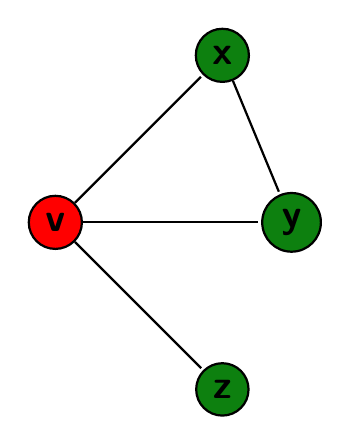
\begin{tikzpicture}[-,>=stealth',shorten >=1pt,auto,node distance=3cm,
  thick,main node/.style={circle,fill=red,draw,font=\sffamily\Large\bfseries},
        others node/.style={circle,fill=cgreen,draw,font=\sffamily\Large\bfseries}]
  \node[main node] (1) {v};
  \node[others node] (2) [above right of=1] {x};
  \node[others node] (3) [right of=1] {y};
  \node[others node] (4) [below right of=1] {z};
  
  \path[every node/.style={font=\sffamily\small}]
    (1) edge (2)
    (1) edge (3)
    (1) edge (4)
    (2) edge (3);
\end{tikzpicture} \\
\end{minipage}

\newpage

\begin{minipage}{0.5\textwidth}
\underline{\textbf{Buddy}} \cite{A_P_rec} \\ \\
Search two vertices v $\neq$ w with $d_{G}(v) = d_{G}(w) = 3$ such that they share their neighbours. Let x, y and z the neighbours of v and w. \\
Create two bags \{v, x, y, z\} and \{w, x, y, z\}. Create an edge between these bags. \\
Make x, y and z a clique and remove v and w. \\ \\
\underline{implementation detail}: just create one of the bags e.g. that one containing v, Triangle will be appliable on w. \\ 
\end{minipage}
\hspace{2.0cm}
\begin{minipage}{0.5\textwidth}
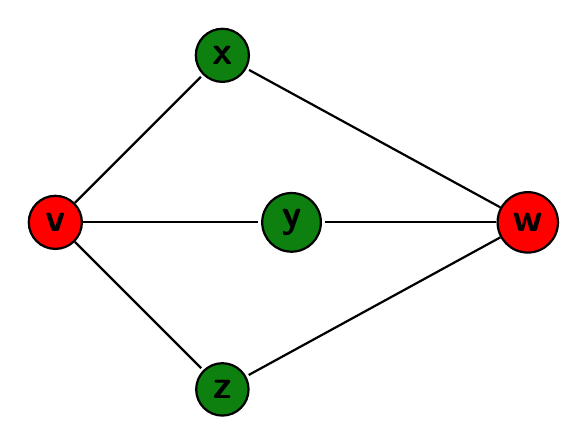
\begin{tikzpicture}[-,>=stealth',shorten >=1pt,auto,node distance=3cm,
  thick,main node/.style={circle,fill=red,draw,font=\sffamily\Large\bfseries},
        others node/.style={circle,fill=cgreen,draw,font=\sffamily\Large\bfseries}]
  \node[main node] (1) {v};
  \node[others node] (2) [above right of=1] {x};
  \node[others node] (3) [right of=1] {y};
  \node[others node] (4) [below right of=1] {z};
  \node[main node] (5) [right of=3] {w};
  
  \path[every node/.style={font=\sffamily\small}]
    (1) edge (2)
    (1) edge (3)
    (1) edge (4)
    (5) edge (2)
    (5) edge (3)
    (5) edge (4);
\end{tikzpicture} \\
\end{minipage}

\vspace*{0.5cm}

\begin{minipage}{0.5\textwidth}
\underline{\textbf{Cube}} \cite{A_P_rec} \\ \\
Iterate through all vertices d $\in$ G. \\
If $d_{G}(d) == 3$: \\
Let x, y and z the neighbours of d. Check if they all have degree 3 in G. If this is the case, test if each two have exactly one neighbour in common (which will be a, b and c). Finally check for the remaining edges and non-edges as shown below. 
Create the bags \{x, a, b, d\}, \{y, a, c, d\} and \{z, b, c, d\}. Create an edge between these bags. \\
Make $\{a,b,c,d\}$ a clique and remove x, y and z.\\  \\
\underline{implementation detail}: just create one of the bags e.g. \{z ,b, c, d\}, Triangle will be appliable on the rest. \\ 
\end{minipage}
\hspace{2.0cm}
\begin{minipage}{0.5\textwidth}
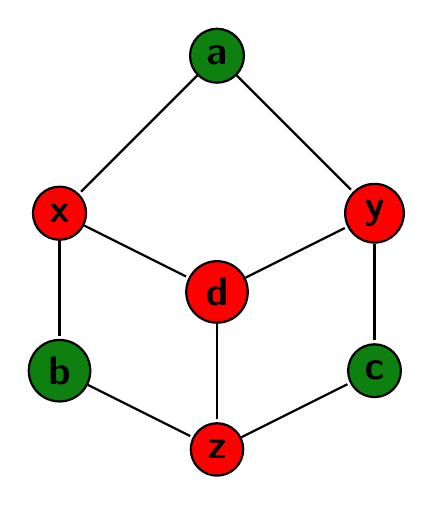
\begin{tikzpicture}[-,>=stealth',shorten >=1pt,auto,node distance=3cm,
  thick,main node/.style={circle,fill=red,draw,font=\sffamily\Large\bfseries},
        others node/.style={circle,fill=cgreen,draw,font=\sffamily\Large\bfseries}]
  \node[others node] (1) at (1,0){a};
  \node[main node] (2) at (-1,-2){x};
  \node[main node] (3) at (1,-3){d};
  \node[main node] (4) at (3,-2){y};
  \node[others node] (5) at (-1,-4) {b};
  \node[main node] (6) at (1, -5) {z};
  \node[others node] (7) at(3,-4) {c};
  
  \path[every node/.style={font=\sffamily\small}]
    (1) edge (2)
    (1) edge (4)
    (2) edge (3)
    (2) edge (5)
    (3) edge (4)
    (3) edge (6)
    (4) edge (7)
    (5) edge (6)
    (6) edge (7);
\end{tikzpicture} \\
\end{minipage}

\vspace*{0.5cm}

\begin{minipage}{0.5\textwidth}
\underline{\textbf{Simplicial}} \\ \\
Search a vertex v, such that the neighbours of v including v induce a clique (pairwise are connected by an edge). 
Create a bag containing this clique and remove v. \\
\end{minipage}
\hspace{2.0cm}
\begin{minipage}{0.5\textwidth}
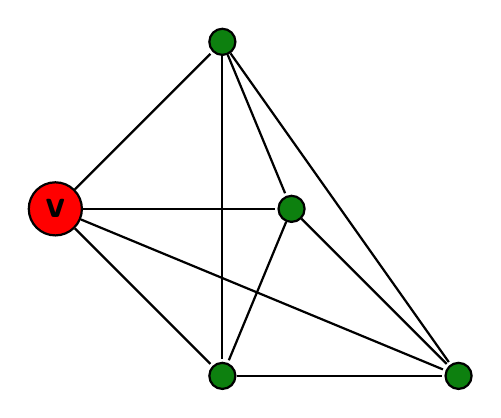
\begin{tikzpicture}[-,>=stealth',shorten >=1pt,auto,node distance=3cm,
  thick,main node/.style={circle,fill=red,draw,font=\sffamily\Large\bfseries},
        others node/.style={circle,fill=cgreen,draw,font=\sffamily\Large\bfseries}]
  \node[main node] (1) {v};
  \node[others node] (2) [above right of=1] {};
  \node[others node] (3) [right of=1] {};
  \node[others node] (4) [below right of=1] {};
  \node[others node] (5) [below right of=3] {};
  
  \path[every node/.style={font=\sffamily\small}]
    (1) edge (2)
    (1) edge (3)
    (1) edge (4)
    (1) edge (5)
    (2) edge (3)
    (2) edge (4)
    (2) edge (5)
    (3) edge (4)
    (3) edge (5)
    (4) edge (5);
\end{tikzpicture} \\
\end{minipage}

\newpage

\begin{minipage}{0.5\textwidth}
\underline{\textbf{Almost Simplicial}} \cite{B_tc3} \\ \\
Search a vertex v, such that the neighbours of v, except exactly one vertex w, called the special neighbour of v, induce a clique. \\ \\
\underline{implementation detail}: If \{u, w\} $\notin$ E(G), u or w is the special neighbour of v, depending on how many edge misses occur. If there would be more than one special neighbour of v, the rule is not applicable. \\
\end{minipage}
\hspace{2.0cm}
\begin{minipage}{0.5\textwidth}
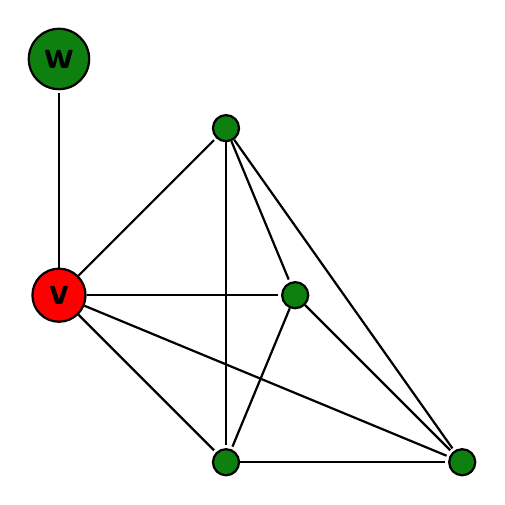
\begin{tikzpicture}[-,>=stealth',shorten >=1pt,auto,node distance=3cm,
  thick,main node/.style={circle,fill=red,draw,font=\sffamily\Large\bfseries},
        others node/.style={circle,fill=cgreen,draw,font=\sffamily\Large\bfseries}]
  \node[main node] (1) {v};
  \node[others node] (2) [above right of=1] {};
  \node[others node] (3) [right of=1] {};
  \node[others node] (4) [below right of=1] {};
  \node[others node] (5) [below right of=3] {};
  \node[others node] (6) [above of=1] {w};
  
  \path[every node/.style={font=\sffamily\small}]
    (1) edge (2)
    (1) edge (3)
    (1) edge (4)
    (1) edge (5)
    (1) edge (6)
    (2) edge (3)
    (2) edge (4)
    (2) edge (5)
    (3) edge (4)
    (3) edge (5)
    (4) edge (5);
\end{tikzpicture}
\end{minipage}

\begin{table}[h!]
\begin{tabular}{|l|l|}
\hline 
rule & complexity \\
\hline  
Islet & $O(|V|)$ \\
Twig &$O(|V|)$ \\
Series &$O(|V|)$ \\
Triangle &$O(|V|)$ \\
Buddy &$O(|V|^2)$ \\
Cube &$O(|V|)$ \\
Simplicial vertex &$O(|V|^2)$ \\
Almost simplicial vertex &$O(|V|^2)$ \\
glueing a bag &$O(|V|*tw(G))$ \\
\hline
\end{tabular}
\caption{Asymtotic runtime for identifying, if a specific rule is applicable on a graph and, if this is the case, applying this rule. $|V|$ denotes the number of vertices of the input graph.} 
\end{table}

\subsection{Algorithm}

The main algorithm successivly tests if at least one rule is applicable on the input graph G and if this is the case reduces G according to that rule. If no rule is applicable and the processed graph is not the empty graph, another algorithm for computing tree decompositions can be started on the reduced instance of G. \\
Since each rule creates a clique when applied and a clique must be contained in some bag, the bag corresponding to the rule (without the removed vertex) can be glued with at least one bag, that will be produced in future and containes the mentioned clique. \\ 
Assuming we have a tree decomposition of the remaining graph, it is sufficient to glue the current considered bag with exactly one bag, that containes this clique. The following algorithm processes recursivly to do so: \\

\newpage

\begin{algorithm}
\caption{tw-preprocessing}
\begin{algorithmic}
\Procedure{preprocessing}{graph G, tree decomposition T}
\If {$|V(G)|$ == 0}
\State \Return T
\EndIf
\State {}
\State {bag := $\emptyset$}
\State {}
\State {//a rule modifies G and fills bag if it is applicable}
\If {Islet(G, bag) $||$ ... $||$ AlmostSimplicial(G, bag)}
\State {preprocessing(G, T)}
\State {create a vertex in T, labeled with bag and connect bag without the preprocessed}
\State { vertex with exactly one bag in T according to set containment \\}
\Return
\EndIf
\If {no rule can be applied and G is not the empty graph}
\State {//the input graph is not fully reducable with the reduction rules and tw(G) $>$ 3}
\State {//use another algorithm to fully decompose the possibly reduced graph G}
\EndIf
\EndProcedure
\end{algorithmic}
\end{algorithm}	

\vspace*{3mm}

Short circuit evaluation results in reduction of G by the first applicable rule. The chronological order of the rules has been choosen by increasing treewidth, applicability and complexity and is as follows: Islet, Twig, Series, Triangle, Buddy, Cube AlmostSimplicial. The whole preprocessing can be done in time $O(|V|^{3})$: \\
Checking if a rule is applicable can be done in time $O(|V|^{2})$, which will be done with at the worst each rule. Since a rule removes at least one vertex, the empty graph is reached after at most $|V|$ reductions or the algorithm states, that no rule can be applied earlier. Glueing a bag costs $O(|V|^{2})$: When bags are stored as sets, a comparison can be done in linear time in the smaller sized bag by merging. The algorithm tests all at most $|V|$ bags in the so far obtained tree decomposition for containing the clique, that has been produced by applying a reduction, and adds an edge in the \enquote{partial tree decomposition}, if this is the case. \\ 

\newpage

\subsection{Results}

Figure 1 shows the proportion of rules applied on the tested graphs. Figure 2 shows some efficency results of the test run. 11 of the 1817 control flow graphs could not fully preprocessed to an empty graph. Figures 3 to 13 show the reduced graphs of these instances.

\vspace*{5mm}

\begin{table}[h!]
\small{
\begin{tabular}{|l|l|l|l|l|l|l|}
\hline 
package & \#graphs & avg width & max width & \#not fully prep. & avg reduction & total time[ms] \\
\hline 
\hline 
stdlib & 142 & 1.85211 & 4 & 0 & 1 & 24.492 \\
contiki & 1082 & 1.69501 & 4 & 9 & 1 & 274.131 \\
fuzix & 529 & 1.95841 & 4 & 2 & 1 & 116.363 \\
coremark & 42 & 1.64286 & 3 & 0 & 1 & 18.126 \\
whetstone & 7 & 1.42857 & 2 & 0 & 1 & 3.831 \\
dhrystone & 15 & 1.66667 & 2 & 0 & 1 & 4.691 \\
dimacs & 82 & 8.65854 & 34 & 79 & 0.47561 & 345.34 \\
zoo & 150 & 0.886667 & 14 & 123 & 0.26 & 220.73 \\

\hline
\end{tabular}
}
\caption{...}
\end{table}

As excepted, preprocessing is of inconsiderable use for the DIMACS graphs: the preprocessing rules are, except the simplicial and almost simplicial rule, degree based, such that they are not applicable on graphs with high minimal degree. \\
On the contrary, all but 11 control flow graphs could be fully reduced to the empty graph by preprocessing: Preprocessing could be a part of a standard-approach to gain tree decompositions of control flow graphs. Now, for the 11 graphs, we have a smaller instance and, in addition, a lower bound on the treewidth of these.

\subsection{Usage}

\begin{lstlisting}[mathescape]
#include<tdlib/preprocessing.hpp>

graph_t G;
tree_dec_t T;

std::vector<boost::tuple<unsigned int,
            std::set<unsigned int> > > bags;
treedec::preprocessing(G, bags);
treedec::glue_bags(bags, T);
\end{lstlisting}

If $G$ is not reducable to the empty graph by preprocessing, a treedecomposition of $G$ (after preprocessing) has to be computed in order to obtain a valid treedecomposition of the input graph.

\begin{comment}

%\section{Some preprocessing rules for tree width 4}

%\subsection{Rules}

\underline{\textbf{simple Y-$\Delta$-reductions}} \\

\underline{\textbf{YO}} \\

Iterate through all vertices x $\in$ G. \\
If $d_{G}(x) = 3$: \\
For all (at most 3) choices of neighbours y, z of x, such that $d_{G}(z) = d_{G}(y) = 3$: Let $N_{G}(z) \backslash \{x\} = \{s,t\}$ and $N_{G}(y) \backslash \{x\} = \{m,n\}$. If
\begin{itemize}[noitemsep,topsep=1pt,parsep=0pt,partopsep=1pt] 
\item s = m, t $\neq$ n then a:=s, c:=t, b:=n
\item s = n, or t = m or t = n: analog 
\item otherwise continue with the next choice of y and z.
\end{itemize}
Let d:=$N_{G}(x) \backslash \{y,z\}$. If the edges between vertices in $\{a,b,c,d\}$ are connected as shown in the figure below, then add a bag containing $\{x, y, z, d\}$, make $\{x,y,z,d\}$ a clique and remove x.  

\vspace*{0.5cm}

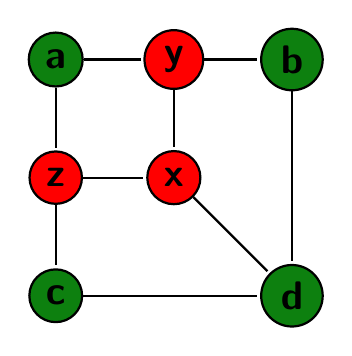
\begin{tikzpicture}[-,>=stealth',shorten >=1pt,auto,node distance=1.5cm,
  thick,main node/.style={circle,fill=red,draw,font=\sffamily\Large\bfseries},
        others node/.style={circle,fill=cgreen,draw,font=\sffamily\Large\bfseries}]
  \node[others node] (1) {a};
  \node[main node] (2) [below of=1] {z};
  \node[main node] (3) [right of=1] {y};
  \node[main node] (4) [right of=2] {x};
  \node[others node] (5) [below of=2] {c};
  \node[others node] (6) [right of=3] {b};
  \node[others node] (7) [right of=5, xshift=1.5cm] {d};
  
  \path[every node/.style={font=\sffamily\small}]
    (1) edge (2)
    (1) edge (3)
    (2) edge (4)
    (2) edge (5)
    (3) edge (4)
    (3) edge (6)
    (4) edge (7)
    (5) edge (7)
    (6) edge (7);
\end{tikzpicture} \\

\underline{\textbf{H7}} \\

Iterate through all vertices x $\in$ G. \\
If $d_{G}(x) = 3$: \\
For all (at most 3) possibilities of choosing y: \\
If $d_{G}(y) = 3$: Let $\{m,n\} = N_{G}(y) \backslash \{x\}$, $\{s,t\} = N_{G}(x) \backslash \{y\}$. If:
\begin{itemize}[noitemsep,topsep=1pt,parsep=0pt,partopsep=1pt] 
\item $\{m, s\} \in E(G)$, then a:=n, b:=s, c:=m, d:=t 
\item $\{m, t\} \in E(G)$ or $\{n, s\} \in E(G)$ or $\{n, t\} \in E(G)$: analogous
\item otherwise continue with the next choice of y.
\end{itemize} 
If exactly the edges shown in the figure below exist, then add a bag containing $\{x, y, b, d\}$, make $\{x,y,b,d\}$ a clique and remove x.  

\vspace*{0.5cm}

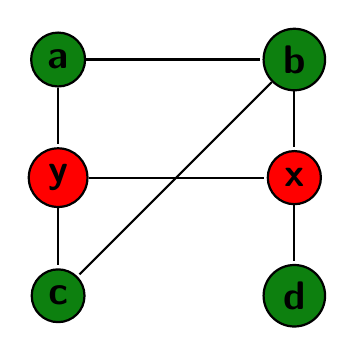
\begin{tikzpicture}[-,>=stealth',shorten >=1pt,auto,node distance=1.5cm,
  thick,main node/.style={circle,fill=red,draw,font=\sffamily\Large\bfseries},
        others node/.style={circle,fill=cgreen,draw,font=\sffamily\Large\bfseries}]
  \node[others node] (1) {a};
  \node[main node] (2) [below of=1] {y};
  \node[others node] (3) [right of=1, xshift=1.5cm] {b};
  \node[main node] (4) [right of=2, xshift=1.5cm] {x};
  \node[others node] (5) [below of=2] {c};
  \node[others node] (6) [right of=5, xshift=1.5cm] {d};
  
  \path[every node/.style={font=\sffamily\small}]
    (1) edge (2)
    (1) edge (3)
    (2) edge (4)
    (2) edge (5)
    (3) edge (4)
    (3) edge (5)
    (4) edge (6);
\end{tikzpicture} \\

\vspace*{0.5cm}

\underline{\textbf{TO}} \\

\vspace*{0.3cm}

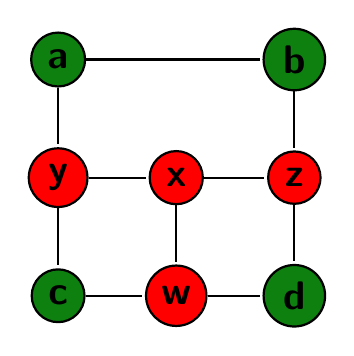
\begin{tikzpicture}[-,>=stealth',shorten >=1pt,auto,node distance=1.5cm,
  thick,main node/.style={circle,fill=red,draw,font=\sffamily\Large\bfseries},
        others node/.style={circle,fill=cgreen,draw,font=\sffamily\Large\bfseries}]
  \node[others node] (1) {a};
  \node[main node] (2) [below of=1] {y};
  \node[others node] (3) [right of=1, xshift=1.5cm] {b};
  \node[main node] (4) [right of=2] {x};
  \node[main node] (5) [right of=4] {z};
  \node[others node] (6) [below of=2] {c};
  \node[main node] (7) [right of=6] {w};
  \node[others node] (8) [right of=7] {d};
  
  \path[every node/.style={font=\sffamily\small}]
    (1) edge (2)
    (1) edge (3)
    (2) edge (4)
    (2) edge (6)
    (3) edge (5)
    (4) edge (5)
    (4) edge (7)
    (5) edge (8)
    (6) edge (7)
    (7) edge (8);
\end{tikzpicture} \\

\vspace*{1cm}

\underline{\textbf{YI}} \\

Note, that \enquote{YI := YO - $\{c,d\}$ - $\{b,d\}$ + $\{c,b\}$}. Check the applicability of this rule analogous to YO. If this rule can be applied, eliminate x, which results in the bag $\{x,y,z,d\}$. \\

\vspace*{0.5cm}

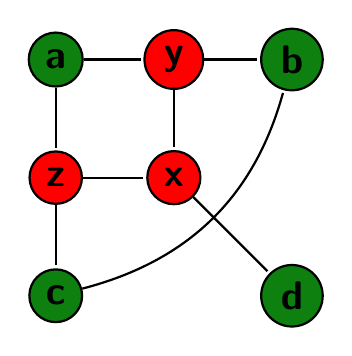
\begin{tikzpicture}[-,>=stealth',shorten >=1pt,auto,node distance=1.5cm,
  thick,main node/.style={circle,fill=red,draw,font=\sffamily\Large\bfseries},
        others node/.style={circle,fill=cgreen,draw,font=\sffamily\Large\bfseries}]
  \node[others node] (1) {a};
  \node[main node] (2) [below of=1] {z};
  \node[main node] (3) [right of=1] {y};
  \node[main node] (4) [right of=2] {x};
  \node[others node] (5) [below of=2] {c};
  \node[others node] (6) [right of=3] {b};
  \node[others node] (7) [right of=5, xshift=1.5cm] {d};
  
  \path[every node/.style={font=\sffamily\small}]
    (1) edge (2)
    (1) edge (3)
    (2) edge (4)
    (2) edge (5)
    (3) edge (4)
    (3) edge (6)
    (4) edge (7)
    (5) edge [bend right] (6);
    
\end{tikzpicture} \\

\underline{\textbf{Ladder reductions}} \\

\underline{\textbf{L1}} \\

Iterate through all vertices x $\in$ G. If $d_{G}(x) = 3$: \\
For all choices of two neighbours $v_{3}, v_{4}$ of x, such that both have degree 3 and share a vertex y, y $\neq$ x, $d_{G}(y) = 3$:  Let $v_{1}$ be the vertex in $N_{G}(v_{3}) \backslash \{x, y\}$. Define  $v_{2}$, $v_{4}$ and $v_{5}$ analogous due to the information of the neighbourhood of x, y and $v_{4}$. Finally, check, if vertices in $\{v_{1}, v_{2}, v_{5}, v_{6}\}$ are connected as shown below. If this is the case, eliminate x and y. \\

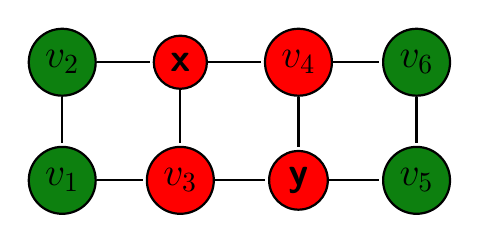
\begin{tikzpicture}[-,>=stealth',shorten >=1pt,auto,node distance=1.5cm,
  thick,main node/.style={circle,fill=red,draw,font=\sffamily\Large\bfseries},
        others node/.style={circle,fill=cgreen,draw,font=\sffamily\Large\bfseries}]
  \node[others node] (1) {$v_{2}$};
  \node[others node] (2) [below of=1] {$v_{1}$};
  \node[main node] (3) [right of=1] {x};
  \node[main node] (4) [right of=2] {$v_{3}$};
  \node[main node] (5) [right of=3] {$v_{4}$};
  \node[main node] (6) [right of=4] {y};
  \node[others node] (7) [right of=5] {$v_{6}$};
  \node[others node] (8) [right of=6] {$v_{5}$};
  
  \path[every node/.style={font=\sffamily\small}]
    (1) edge (2)
    (1) edge (3)
    (2) edge (4)
    (3) edge (4)
    (3) edge (5)
    (4) edge (6)
    (5) edge (6)
    (5) edge (7)
    (6) edge (8)
    (7) edge (8);
\end{tikzpicture} \\

\vspace*{0.5cm}

\underline{\textbf{L2}} \\

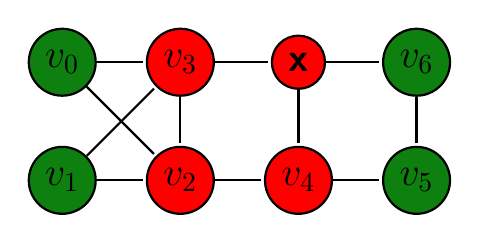
\begin{tikzpicture}[-,>=stealth',shorten >=1pt,auto,node distance=1.5cm,
  thick,main node/.style={circle,fill=red,draw,font=\sffamily\Large\bfseries},
        others node/.style={circle,fill=cgreen,draw,font=\sffamily\Large\bfseries}]
  \node[others node] (1) {$v_{0}$};
  \node[others node] (2) [below of=1] {$v_{1}$};
  \node[main node] (3) [right of=1] {$v_{3}$};
  \node[main node] (4) [right of=2] {$v_{2}$};
  \node[main node] (5) [right of=3] {x};
  \node[main node] (6) [right of=4] {$v_{4}$};
  \node[others node] (7) [right of=5] {$v_{6}$};
  \node[others node] (8) [right of=6] {$v_{5}$};
  
  \path[every node/.style={font=\sffamily\small}]
    (1) edge (3)
    (1) edge (4)
    (2) edge (3)
    (2) edge (4)
    (3) edge (4)
    (3) edge (5)
    (4) edge (6)
    (5) edge (6)
    (5) edge (7)
    (6) edge (8)
    (7) edge (8);
\end{tikzpicture} \\

\newpage

\underline{\textbf{L3}} \\

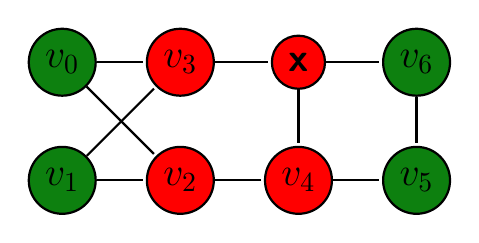
\begin{tikzpicture}[-,>=stealth',shorten >=1pt,auto,node distance=1.5cm,
  thick,main node/.style={circle,fill=red,draw,font=\sffamily\Large\bfseries},
        others node/.style={circle,fill=cgreen,draw,font=\sffamily\Large\bfseries}]
  \node[others node] (1) {$v_{0}$};
  \node[others node] (2) [below of=1] {$v_{1}$};
  \node[main node] (3) [right of=1] {$v_{3}$};
  \node[main node] (4) [right of=2] {$v_{2}$};
  \node[main node] (5) [right of=3] {x};
  \node[main node] (6) [right of=4] {$v_{4}$};
  \node[others node] (7) [right of=5] {$v_{6}$};
  \node[others node] (8) [right of=6] {$v_{5}$};
  
  \path[every node/.style={font=\sffamily\small}]
    (1) edge (3)
    (1) edge (4)
    (2) edge (3)
    (2) edge (4)
    (3) edge (5)
    (4) edge (6)
    (5) edge (6)
    (5) edge (7)
    (6) edge (8)
    (7) edge (8);
\end{tikzpicture} \\

\vspace*{0.5cm}

\underline{\textbf{L4}} \\

Test the applicability of this rule for fixed $v_{4}$ instead of fixed x. The cases, that have to be checked are the same as in some simple Y-$\Delta$-reductions. Eliminate x, if this rule is applicable.\\

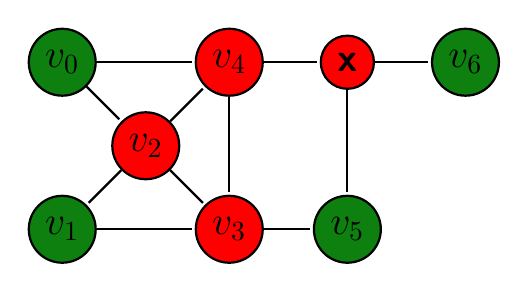
\begin{tikzpicture}[-,>=stealth',shorten >=1pt,auto,node distance=1.5cm,
  thick,main node/.style={circle,fill=red,draw,font=\sffamily\Large\bfseries},
        others node/.style={circle,fill=cgreen,draw,font=\sffamily\Large\bfseries}]
  \node[others node] (1) {$v_{0}$};
  \node[main node] (2) [below right of=1] {$v_{2}$};
  \node[others node] (3) [below left of=2] {$v_{1}$};
  \node[main node] (4) [above right of=2] {$v_{4}$};
  \node[main node] (5) [below right of=2] {$v_{3}$};
  \node[main node] (6) [right of=4] {x};
  \node[others node] (7) [right of=5] {$v_{5}$};
  \node[others node] (8) [right of=6] {$v_{6}$};
  
  \path[every node/.style={font=\sffamily\small}]
    (1) edge (2)
    (1) edge (4)
    (2) edge (3)
    (2) edge (4)
    (2) edge (5)
    (3) edge (5)
    (4) edge (5)
    (4) edge (6)
    (5) edge (7)
    (6) edge (7)
    (6) edge (8); 
\end{tikzpicture} \\


%\subsection{Results}

We tested the partial set of reduction rules for treewidth 4 on the eleven not by rules for treewidth at most 3 fully reducable graph instances. Even though the reductions seem to be of a very special structure, some rules could be applied (2x H7, 3x YI). As one can see in further sections, $handle\_input$, $psock\_readbuf\_len$, $psock\_send$ and $irc\_process$ have treewidth 4 and hence can be reduced to the empty graph by not implemented reduction rules for treewidth at most 4. Note, that a tw4-reduction can make it possible to apply a tw3-reduction such as Triangle.

\end{comment}

\newpage

\section{Lower Bounds}

Lower bounds on treewidth are of multiple use: First, to provide a better start for exact algorithm, that usually increment an integer until this one matches the treewidth, such that resultless calls could be avoided. Second, to estimate the use of just trying to find a tree decomposition by an exact algorithm with respect to an upper bound: if the gap is too high, one may not use an exact algorithm because of inacceptable running time. Third, one could check, if heuristics, that give tree decompositions of graphs, give exact ones, by comparing the width of the returned tree decompositions with the computed lower bound. If these are equal, we have a tree decomposition of exact width. \\

\subsection{Degree Based}

\underline{\textbf{delta}} \cite{B_lb_db} \\ \\
$\delta(G) := min_{v \in V(G)}d_{G}(v)$ \\

\vspace*{2mm}


\underline{\textbf{delta2}} \cite{B_lb_db} \\ \\
$\delta_{2}(G) := min \{ d_{G}(v) : v \in V(G) \land \exists w \in V(G) : d_{G}(w) \leq d_{G}(v) \}$ \\

\vspace*{2mm}


\underline{\textbf{gamma}} \cite{B_lb_db} \\ \\


$ \gamma (G) := \{ 
  \begin{array}{l l}
    |V(G)| -1  & \quad \text{if G is complete}\\
    min_{u,v \in V(G), \{u,v \} \notin E(G)} max \{ d_{G}(v), d_{G}(w) \} & \quad \text{otherwise}
  \end{array}$ \\
  
\begin{algorithm}
\begin{algorithmic}[1]
\State {let DS := ($v_{1}$,..,$v_{n}$), n := $|V(G)|$ with  $d_{G}(v_{1}) \leq .. \leq d_{G}(v_{n})$} 
\For {$v_{1}$,..,$v_{i}$,..,$v_{n}$ in DS}
\For {$v_{1}$,..,$v_{j}$,..,$v_{i-1}$ in DS}
\If  {$\{v_{j}, v_{i}\} \notin E(G)$}
\State {\Return $d_{G}(v_{i})$}
\EndIf
\EndFor
\EndFor
\State {\Return $|V(G)|$ -1}
\end{algorithmic}
\end{algorithm}

\vspace*{2mm}

\underline{\textbf{deltaD}} \cite{B_lb_db, CC_lb_nw} \\ \\
$ \delta D(G) := max_{G'} \{ \delta (G') : G' \subseteq G \}$ \\

\begin{algorithm}
\begin{algorithmic}[1]
\State {maxmin = 0}
\State {H := G}
\While {$V(H) \neq \emptyset$}
\State {v\_min = minimum degree vertex in H}
\State {maxmin = $max \{$maxmin, $d_{H}($v\_min$) \}$}
\State {$H := H - \{$ v\_min $\}$}
\EndWhile
\State {\Return maxmin}
\end{algorithmic}
\end{algorithm}

\newpage

\underline{\textbf{delta2D}} \cite{B_lb_db} \\ \\
$ \delta_{2} D(G) := max_{G'} \{ \delta_{2} (G') : G' \subseteq G \}$ \\

\begin{algorithm}
\begin{algorithmic}[1]
\State {maxmin = 0}
\For {all $v \in V(G)$}
\State {H := G}
\While {$V(H) \neq \emptyset$}
\State {w := $min \{ s \in V(H) : s \neq v \land \neg \exists t \in V(H) - \{ v \} : d_{H}(t) < d_{H}(s) \}$}
\State {maxmin = $max \{$maxmin,$|N_{H}(w)| \}$}
\State {H := H - $\{w \}$}
\EndWhile
\EndFor
\State {\Return maxmin}
\end{algorithmic}
\end{algorithm}

\vspace*{2mm}
        
\underline{\textbf{gammaD}} \cite{B_lb_db} \\ \\
$ \gamma D(G) := max_{H} \{ \gamma (H) : H \subseteq G \}$ \\

\begin{algorithm}
\begin{algorithmic}[1]
\State {let i be the index of the returned element of $\gamma (G)$}
\State {determine $\gamma (H_{i})$ of one of the following subgraphs:}
\State {\textbf{$<\gamma D-left>$}}
\State {$H_{1}$ := $G[V(G) - \{v_{1},..,v_{i-1} \}]$}
\State {\textbf{$<\gamma D-right>$}}
\State {$H_{2}$ := $G[V(G) - \{v_{i} \}]$}
\State {\textbf{$<\gamma D-min-e>$}}
\State {$H_{3}$ := if $|E(H_{1})| \geq |E(H_{2})|$ then $H_{1}$ else $H_{2}$}
\end{algorithmic}
\end{algorithm}

\underline{\textbf{deltaC}} \cite{B_lb_db,B_tc2, GD_lb_bb} \\ \\
$ \delta C(G) := max_{H} \{ \delta (H) : H \preceq G \}$ \\
\begin{lstlisting}[mathescape]
maxmin = 0
G* := G
while |V(G*)| $\geq$ 2:
    v := minimum degree vertex in G*
    N := $N_{G*}(v)$
    maxmin = $max \{$maxmin,$|N_{G*}(v)| \}$
    min-d:
        w := minimum degree vertex in N
    max-d:
        w := maximum degree vertex in N
    least-c:
        w := $v \in N$: #edges, which will be 
                   deleted by contracting $\{ v, w \}$ is minimal
    G* := G*/$\{ v, w \}$
return maxmin
\end{lstlisting}

\subsection{Improved Graphs}

references: \cite{B_tc2, B_lb_ne, CC_lb_nw, B_lb_lt, B_lb_ct} \\

\underline{\textbf{neighbour improved graphs}}
\begin{lstlisting}[mathescape]
for all $\{ v,w \} : \{ v,w \} \notin E(G)$: 
    if $N_{G}(v) \cap N_{G}(w) \geq k$:
        G* := (V(G), E(G) $\cup$ $\{\{ v,w \}\}$)
\end{lstlisting}

\vspace*{3mm}

\underline{\textbf{path improved graphs}}
\begin{lstlisting}[mathescape]
for all $\{ v,w \} : \{ v,w \} \notin E(G)$: 
    if #disjoint paths from v to w $\geq k$:
        G* := (V(G), E(G) $\cup$ $\{\{ v,w \}\}$)
\end{lstlisting} 

\vspace*{0.5cm}

\textbf{LBN/LBP}
\begin{lstlisting}[mathescape]
let X be an algorithm to determine a lower bounds of tw(G)
LB := X(G)
H := LB+1-neighbour(path)-improved-graph
changed = True
while changed:
    changed := False
    newLB := X(H)
    if newLB > LB:
        LB := LB + 1
        changed := True
return LB
\end{lstlisting}

\vspace*{5mm}

All degree-based lower bounds mentioned above can be computed based on the improved graph.

\newpage

\subsection{Maximum Cardinality Search}

The algorithm is as follows: Mark an an arbitrary vertex $v_{0} \in G$. While there are unmarked vertices, mark the vertex with the maximum number of marked neighbours next. Let $v_{i}$ be the choosen vertex in iteration i. We call the number of marked neighbours of $v_{i}$ the visited degree of $v_{i}$. The maximum over all visited degrees is a lower bound to the treewidth of G. \\

Each maximum-cardinality-ordering $\pi$ provides an lower bound according to treewidth. Due to NP-completeness of finding a largest maximum-cardinality-ordering there exists following heuristics: \\
(1) proceed with the first visited vertex with most marked neighbours \\
(2) proceed with an arbitary vertex with most marked neighbours \\
(3) apply MCS to G for each start vertex $v_{0}$ with heuristics (1) or (2) \\ 

MCS can be combinated with contration using the most effective heuristic least-c. For  the choice of the next edge that will be contracted, there are the heuristics:
\begin{itemize}
\item \underline{\textbf{min-deg}}:  contract an edge between an minimum-degree-vertex v and a vertex w choosen by least-c 
\item \underline{\textbf{last-mcs}}: contract an edge between the last visited vertex in the previous MCS-run and a vertex w choosen by least-c 
\item \underline{\textbf{max-mcs}}: contract an edge between the vertex with maximum-visited-degree in the previous MCS-run and a vertex w choosen by least-c
\end{itemize}

\subsection{Results}

We tested all lower bound-algorithms on the reduced instances of the not fully preprocessable control flow graphs. \\

\begin{table}[h!]
\small
\centering
\begin{tabular}{|l|r|}
\hline 
algorithm & complexity \\
\hline  
\hline
delta  & $O(|V|)$ \\
delta2 & $O(|V|)$ \\
gamma  & $O(|V|+|E|)$ \\
\hline 
deltaD & $O(|V|^2)$ \\
delta2D & $O(|V|^3)$ \\
gammaD-left &  $O(|V|+|E|)$ \\
gammaD-right &  $O(|V|+|E|)$ \\
gammaD-min-e &  $O(|V|+|E|)$ \\
\hline 
deltaC-min-d &  $O(|V| \cdot(|V| + \Delta(G))$ \\
deltaC-max-d &  $O(|V| \cdot(|V| + \Delta(G))$ \\
deltaC-least-c &  $O(|V| \cdot(|V| + \Delta(G))$ \\
\hline 
\end{tabular}
\caption{Asymptotic runtime for applying an lower bound-algorithm on a graph. (1/2)}
\end{table}

\newpage

\begin{table}[h!]
\small
\centering
\begin{tabular}{|l|r|}
\hline 
algorithm & complexity \\
\hline  
\hline
neighbour-improved graph & $O(|V|^3)$ \\
path-improved graph & $O(|V|^2 \cdot (tw(G) \cdot (|V| + |E|))$ \\
\hline 
\hline 
MCS-single &  $O(|V|+|E|)$\\
MCS-all-start & $O(|V| \cdot(|V|+|E|))$\\
MCSC-min-deg &  \\
MCSC-last-mcs &  \\
MCSC-max-mcs &  \\
\hline 
\end{tabular}
\caption{Asymptotic runtime for applying an lower bound-algorithm on a graph. (2/2)}
\end{table}

\begin{table}[h!]
\small
\centering
\begin{tabular}{|l|l|l|l|l|l|l|}
\hline
name & delta & delta2 & gamma & deltaD & delta2D & gammaD-left \\
\hline
\hline
contiki\_contikimac\_powercycle & 3 & 3 & 3 & 3 & 4 & 3 \\
contiki\_dhcpc\_handle\_dhcp & 3 & 3 & 3 & 3 & 3 & 3 \\
contiki\_ircc\_handle\_connection & 3 & 3 & 3 & 3 & 3 & 3 \\
contiki\_ircc\_handle\_input & 3 & 3 & 3 & 3 & 3 & 3 \\
contiki\_lpp\_dutycycle & 3 & 3 & 3 & 3 & 3 & 3 \\
contiki\_psock\_psock\_readbuf\_len & 4 & 4 & 4 & 4 & 4 & 4 \\
contiki\_psock\_psock\_send & 3 & 3 & 3 & 3 & 3 & 3 \\
contiki\_shell-irc\_process\_thread\_shell\_irc\_process & 3 & 3 & 3 & 3 & 3 & 3 \\
contiki\_uip\_uip\_process & 3 & 4 & 4 & 4 & 4 & 4 \\
fuzix\_vfprintf\_vfprintf & 3 & 3 & 3 & 3 & 4 & 4 \\
fuzix\_vfscanf\_vfscanf & 3 & 3 & 4 & 4 & 4 & 4 \\

\hline
\end{tabular}
\caption{Evaluation of degree-based lower bound algorithms on the not by preprocessing fully reducable graphs. (1/2)}
\end{table}

\begin{table}[h!]
\small
\centering
\begin{tabular}{|l|l|l|l|l|l|l|}
\hline
name & gammaD-right & gammaD-min-e & deltaC-min-d & deltaC-max-d & deltaC-leastC \\
\hline
\hline
\input{./Results/3_lb2.tex}
\hline
\end{tabular}
\caption{Evaluation of degree-based lower bound algorithms on the not by preprocessing fully reducable graphs. (2/2)}
\end{table}

\newpage

\begin{table}[h!]
\small
\centering
\begin{tabular}{|l|l|l|l|l|l|l|}
\hline
name & LBNdeltaD & LBNdeltaC & LBNCdeltaD & LBNCdeltaC \\
\hline
\hline
contiki\_contikimac\_powercycle & 3 & 4 & 3 & 4\\
contiki\_dhcpc\_handle\_dhcp & 3 & 5 & 3 & 5\\
contiki\_ircc\_handle\_connection & 3 & 4 & 3 & 4\\
contiki\_ircc\_handle\_input & 4 & 4 & 4 & 4\\
contiki\_lpp\_dutycycle & 3 & 4 & 3 & 4\\
contiki\_psock\_psock\_readbuf\_len & 4 & 4 & 4 & 4\\
contiki\_psock\_psock\_send & 3 & 3 & 3 & 3\\
contiki\_shell-irc\_process\_thread\_shell\_irc\_process & 3 & 3 & 3 & 3\\
contiki\_uip\_uip\_process & 4 & 6 & 4 & 6\\
fuzix\_vfprintf\_vfprintf & 3 & 5 & 3 & 5\\
fuzix\_vfscanf\_vfscanf & 4 & 5 & 4 & 5\\

\hline
\end{tabular}
\caption{Evaluation of improved graph-based lower bound algorithms on the not by preprocessing fully reducable graphs. (1/2)}
\end{table}

\begin{table}[h!]
\small
\centering
\begin{tabular}{|l|l|l|l|l|l|l|}
\hline
name & LBPdeltaD & LBPdeltaC & LBPCdeltaD & LBPCdeltaC \\
\hline
\hline
contiki\_contikimac\_powercycle & 4 & 4 & 4 & 4\\
contiki\_dhcpc\_handle\_dhcp & 4 & 5 & 4 & 5\\
contiki\_ircc\_handle\_connection & 3 & 4 & 3 & 4\\
contiki\_ircc\_handle\_input & 4 & 4 & 4 & 4\\
contiki\_lpp\_dutycycle & 3 & 4 & 3 & 4\\
contiki\_psock\_psock\_readbuf\_len & 4 & 4 & 4 & 4\\
contiki\_psock\_psock\_send & 3 & 3 & 3 & 3\\
contiki\_shell-irc\_process\_thread\_shell\_irc\_process & 3 & 3 & 3 & 3\\
contiki\_uip\_uip\_process & 6 & 6 & 6 & 6\\
fuzix\_vfprintf\_vfprintf & 5 & 5 & 5 & 5\\
fuzix\_vfscanf\_vfscanf & 5 & 5 & 5 & 5\\

\hline
\end{tabular}
\caption{Evaluation of improved graph-based lower bound algorithms on the not by preprocessing fully reducable graphs. (2/2)}
\end{table}

\newpage

\begin{table}[h!]
\small
\centering
\begin{tabular}{|l|l|l|l|l|l|l|}
\hline
name & MCS & MCSC \\
\hline
\hline
\input{./Results/6_lb_mcs.tex}
\hline
\end{tabular}
\caption{Evaluation of MCS-lower bound algorithms on some of the not by preprocessing fully reducable graphs.}
\end{table}

\subsection{Usage}

\begin{lstlisting}[mathescape]
#include<tdlib/lower_bounds.hpp>

graph_t G;

treedec::lb::delta(G);
treedec::lb::delta2(G);
treedec::lb::gamma(G);
treedec::lb::deltaD(G);
treedec::lb::delta2D(G);
treedec::lb::gammaD_left(G);
treedec::lb::gammaD_right(G);
treedec::lb::gammaD_min_e(G);
treedec::lb::deltaC_min_d(G)
treedec::lb::deltaC_max_d(G)
treedec::lb::deltaC_least_c(G)
treedec::lb::LBN_deltaD(G)
treedec::lb::LBN_deltaC(G)
treedec::lb::LBNC_deltaD(G)
treedec::lb::LBNC_deltaC(G)
treedec::lb::LBP_deltaD(G)
treedec::lb::LBP_deltaC(G)
treedec::lb::LBPC_deltaD(G)
treedec::lb::LBPC_deltaC(G)
treedec::lb::MCS(G)
treedec::lb::MCSC(G)
\end{lstlisting}

\newpage

\section{Exact Algorithms}

\begin{definition}
A turn (X, y) $\rightarrow$ (X', y) is monotone in the cops and robbers game on graphs :$\leftrightarrow$ comp(G $\backslash$ X, y) = comp(G $\backslash$ (X $\cap$ X'), y), whereas comp(G $\backslash$ X, y) denotes the component of (G $\backslash$ X), such that y $\in$ (G $\backslash$ X), y $\in$ V(G), for a graph G.
\end{definition}

\subsection{Cops and Robbers: greedy version}

The following algorithm can be started by calling explore\_cutsets(G, $\{v\}$, V(G), empty vector results, k) for k = 0,1,2,.. and computes all necessary information about a tree decomposition of the input graph G of optimal width. After a successful call, a tree decomposition is computed out of the sets in 'results' in linear time. 

\begin{algorithm}[h!]
\caption{greedyCR-decomposition}
\begin{algorithmic}
\Procedure{explore\_cutsets}{graph G, cut, component, results, treewidth lower bound k}
\If {$|cut| > k$}
\State {\Return false}
\EndIf
\If {$|cut| + |component| \leq k+1$}
\State{component = component $\cup$ cut}
\State{results.push(component)}
\State{results.push(cut)}
\State {\Return true}
\EndIf
\State {}
\For {v in component}
\State {extended\_cut = cut $\cup$ $\{v\}$}
\State {new\_comps = components($G[component \backslash \{v\}]$)}
\State {}
\For {$0 \leq i \leq |new\_components|$}
\State {reduced\_cut = vertices in extended\_cut that have a neighbour}
\State {in new\_comps[i]}
\If {!explore\_cutsets(G, reduced\_cut, new\_comps[i], results, k)}
\State {goto the first for-loop}
\EndIf
\State {results.push(reduced\_cut)}
\State {results.push(extended\_cut)}
\State {results.push(cut)}
\EndFor
\If {all recursive calls were successful}
\State {\Return true}
\EndIf
\EndFor
\State {\Return false}
\EndProcedure
\end{algorithmic}
\end{algorithm}

\newpage

\subsection{Cops and Robbers: dynamic version}

\begin{algorithm}[h!]
\caption{dynamicCR-decomposition}
\begin{algorithmic}
\Procedure{CRgreedyDecomp}{graph G}

\If {G is complete or the empty graph}
\State {\Return the trivial decomposition}
\EndIf
\State {}
\State {let W a list of lists, containing a position of cops and the current robber space}
\State {k := lb}
\State {}
\While {true}
\State {k++}
\For {i:=0; i $\leq |V(G)|$; i++}
\If {make\_layer(G, W, V(G), k, i)}
\State {make\_tree\_decomposition(W)}
\State {\Return}
\EndIf
\EndFor
\State {}
\State {clear W}
\EndWhile
\EndProcedure

\State {}

\Procedure{make\_layer}{G, W, V, i}
\State {subs $\gets$ all subsets of V of size k}
\If {i != 0}
  \For {all X $\in$ subs}
    \State {Rcomps $\gets$ components of G $\backslash$ X}
    \State {newR := $\emptyset$}
    \For {all tuples (X', R) in W[i-1]}
      \If {X $->$ X' is monotone with respect to R}
        \State {update newR}
        \State {add (X, newR) to W[i] and install a pointer from X to X'}
        \State {\Return , if $X \cup newR = V(G)$}
      \EndIf
    \EndFor
  \EndFor
\EndIf
\State {}
\State {W := W $\cup \{(sub, \emptyset): sub \in subs\}$}

\EndProcedure
\end{algorithmic}
\end{algorithm}

\newpage

\subsection{Results}

We have evaluated the exact algorithm on the by preprocessing (for treewidth at most 3) reduced instances of the not fully preprocessable graphs. Preprocessing deliveres a lower bound for the reduced instances. After preprocessing the deltaC-least-c heuristic for finding a lower bound on the treewidth of a graph has been used to improve the lower bound from preprocessing. This lower bound is the default lower bound that is used for the exact algorithms. In addition, we tested the runtime of the exact algorithm, when the best lower bound (see section lower bounds) is used.

\begin{table}[h!]
\underline{\textbf{greedyCR}} \\
\begin{tabular}{|l|l|l|l|l|l|l|}
\hline
name & $|V'|$ & $|E'|$ & tw & time[ms] \\
\hline
\hline   
powercycle & 13 & 28 & 5 & 56.388 \\
handle\_dhcp & 39 & 70 & 6 & 4.74801e+07 \\
handle\_connection & 32 & 54 & 4 & 24.504 \\
handle\_input & 19 & 40 & 4 & 3.224 \\
lpp\_dutycycle & 14 & 24 & 5 & 95.085 \\
psock\_readbuf\_len & 6 & 12 & 4 & 0.231 \\
psock\_send & 8 & 12 & 4 & 6.209 \\
irc\_process & 8 & 12 & 4 & 0.389 \\
uip\_process & 19 & 56 & 7 & 102647 \\
vfprintf & 17 & 35 & 6 & 25333.9 \\
vfscanf & 21 & 52 & 6 & 26060.3 \\

\hline
\end{tabular}
\caption{greedyCR with default lower bound.}
\end{table}

The computation on handle\_dhcp needed 0.633976 ms when $lb=6$ was provided, but no lower bound algorithm has returned this lower bound.

\begin{table}[h!]
\underline{\textbf{dynamicCR}} \\
\begin{tabular}{|l|l|l|l|l|l|l|l|}
\hline
name & $|V'|$ & $|E'|$ & tw & time[s] \\
\hline
\hline   
contikimac\_powercycle & 13 & 28 & 5 & 52.81 \\
dhcpc\_handle\_dhcp & 39 & 70 & ? & ? \\
ircc\_handle\_connection & 32 & 54 & ? & ? \\
ircc\_handle\_input & 19 & 40 & 4 & 12336.6(=3.5 hours) \\
lpp\_dutycycle & 14 & 24 & 5 & 1051.89 \\
psock\_readbuf\_len & 6 & 12 & 4 & 0.0001 \\
psock\_send & 8 & 12 & 4 & 0.005 \\
irc\_process & 8 & 12 & 4 & 0.005 \\
uip\_process & 19 & 56 & 7 & 410804(=114 hours) \\
vfprintf & 17 & 35 & 6 & 9257.86(=32 min) \\
vfscanf & 21 & 52 & 6 & ? \\

\hline
\end{tabular}
\end{table}

\newpage

The greedy version uses little memory and works quite well if the input graphs has a vertex ordering that more or less follows the strategy for the cops, that is, one of the first monotone turns, that have been computed, are part of a winning strategy for the cops. \\
The dynamic version uses (in theory) much memory, because in each layer, we have at least $\binom{|V|}{k+1}$ entries. For the tested small graphs, memory usage is not problematic, but the runtime is: We have to check at least ${\binom{|V|}{k+1}}^{2}$ pairs of positions, whether they form a monotone turn (with respect to their robber spaces) or not. \\
For both algorithms, the profit of a good lower bound compensates the running time, that is used for running all possible/the best lower bound algorithms before starting the exact algorithm.

\subsection{Usage}

\begin{lstlisting}[mathescape]
#include<tdlib/exact_cutset.hpp>

graph_t G;
tree_dec_t T;

treedec::exact_decomposition_cutset(G, T)
treedec::exact_decomposition_cutset(G, T, lb) //provided lower bound

#include<tdlib/dynamicCR.hpp>

treedec::exact_decomposition_dynamic(G, T)
treedec::exact_decomposition_dynamic(G, T, lb) //provided lower bound
\end{lstlisting}

\newpage

\section{Approximative Algorithms}

\subsection{Elimination Orderings}

All elimination orderings - an elimination ordering in the pseudocode below is the sequence of v's (Algorithm 4, line 3) along the recursive calls - give a valid tree decomposition, when applied to the corresponding graphs, and hence a upper bound on tree width. Unfortunately, there are $(|V|!)$-many elimination orderings for a graph G on $|V|$ vertices. In this section, we evaluate three heuristics, that provide a valid elimation ordering, ehen applied on a graph. If we have a lower bound on the tree width of a graph, we may be able to value the width of a tree decomposition obtained by a heuristic. Since we computed the tree width of all control flow graphs in the testset by preprocessing or by an exact algorithm, we can observe, whether the heuristics perform well or not on our testset. 

\subsubsection{minDegree-heuristic}

We have implemented and evaluated the well known minDegree-heuristic: \\

\begin{algorithm}
\caption{minDegree-heuristic}
\begin{algorithmic}[1]
\Procedure{minDegree}{graph G, tree decomposition T}
\If {G != $\emptyset$}
\State {let v be a minimal-degree-vertex in G}
\State {make $N_{G}(v)$ a clique}
\State {bag $\gets$ $N_{G}[v]$}
\State {G' := G - $\{v\}$}
\State {}
\State {minDegree(G', T)}
\State {connect bag with T according to set containment}
\EndIf
\EndProcedure
\end{algorithmic}
\end{algorithm}

\vspace*{5mm}

The complexity is $O(|V^{3}(G)|)$: minDegree will be called exactly $|V(G)|+1$ times. Finding a minimal-degree-vertex can be done in time $|V(G)|$, for making $N_{G_{i}}(v)$ a clique, where $G_{i}$ is the graph in the i-th recursive call, at most $|V^{2}(G)|$ edges have to be inserted, since this step can increase the minimal degree of the future graphs. If the bags are given as a set, the glueing step in line 9 can be done in time $|V^{2}(G)|$ by doing a merge on at the worst all bags contained in the current tree decomposition. \\

\newpage

\underline{\textbf{Results}} \\

\begin{table}[h!]
\underline{\textbf{minDegree-heuristic}} \\
\begin{tabular}{|l|l|l|l|l|}
\hline
package & \#graphs & avg width & max width & time[ms] \\
\hline
\hline
stdlib & 142 & 1.85211 & 4 & 13.98 \\
contiki & 1082 & 1.72089 & 8 & 103.931 \\
fuzix & 529 & 1.96975 & 6 & 60.907 \\
coremark & 42 & 1.64286 & 3 & 6.151 \\
whetstone & 7 & 1.42857 & 2 & 1.657 \\
dhrystone & 15 & 1.66667 & 2 & 2.588 \\
dimacs & 82 & 107.524 & 379 & 37576.3 \\
zoo & 150 & 20.54 & 189 & 1389.73 \\

\hline
\end{tabular}
\caption{\small{Results on running the minDegree heuristic.} }
\end{table}

\begin{table}[h!]
\underline{\textbf{preprocessing + minDegree-heuristic}} \\
\begin{tabular}{|l|l|l|l|l|}
\hline
package & \#graphs & avg width & max width & time[ms] \\
\hline
\hline
stdlib & 142 & 1.85211 & 4 & 26.03 \\
contiki & 1082 & 1.71442 & 7 & 279.92 \\
fuzix & 529 & 1.96597 & 6 & 118.385 \\
coremark & 42 & 1.64286 & 3 & 16.968 \\
whetstone & 7 & 1.42857 & 2 & 3.76 \\
dhrystone & 15 & 1.66667 & 2 & 4.647 \\
dimacs & 82 & 107.476 & 379 & 39816.3 \\
zoo & 150 & 20.54 & 189 & 1641.23 \\

\hline
\end{tabular}
\caption{\small{Results on first applying preprocessing, then on the reduced instances the minDegree heuristic.}}
\end{table}

\subsubsection{minFill-heuristic}

We also implemented the fillIn heuristic: Choose a vertex v such that the number of fill edges (edges that have to be added to make the neighbourhood of v a clique) is minimal under all vertices of the graph. \\

\begin{table}[h!]
\underline{\textbf{fillIn-heuristic}} \\
\begin{tabular}{|l|l|l|l|l|}
\hline
package & \#graphs & avg width & max width & time[ms] \\
\hline
\hline
stdlib & 142 & 1.8662 & 4 & 19.066 \\
contiki & 1082 & 1.72643 & 7 & 147.994 \\
fuzix & 529 & 1.99244 & 6 & 85.059 \\
coremark & 42 & 1.69048 & 3 & 8.834 \\
whetstone & 7 & 1.42857 & 2 & 2.375 \\
dhrystone & 15 & 1.66667 & 2 & 3.007 \\
dimacs & 82 & 103.634 & 375 & 4.41383e+06 \\
zoo & 150 & 19.8533 & 177 & 49748.5 \\

\hline
\end{tabular}
\caption{\small{Results on running the fillIn heuristic.} }
\end{table}

\begin{table}[h!]
\underline{\textbf{preprocessing + fillIn-heuristic}} \\
\begin{tabular}{|l|l|l|l|l|}
\hline
package & \#graphs & avg width & max width & time[ms] \\
\hline
\hline
stdlib & 142 & 1.85211 & 4 & 28.247 \\
contiki & 1082 & 1.71165 & 7 & 311.43 \\
fuzix & 529 & 1.96597 & 6 & 123.765 \\
coremark & 42 & 1.64286 & 3 & 14.183 \\
whetstone & 7 & 1.42857 & 2 & 3.788 \\
dhrystone & 15 & 1.66667 & 2 & 4.644 \\
dimacs & 82 & 103.634 & 375 & 4.37127e+06 \\
zoo & 150 & 19.8533 & 177 & 49608.1 \\

\hline
\end{tabular}
\caption{\small{Results on first applying preprocessing, then on the reduced instances the fillIn heuristic.}}
\end{table}


\subsubsection{Thorup's heuristic}

The classic approach to obtaining tree-decompositions of control-flow graphs is Thorup's algorithm \cite{thorup}. Krause has proven, that Thorup's heuristic can produce arbitrary huge tree width \cite{C-tree}. Since Thorup's heuristic is used in sdcc \cite{sdcc}, we compared our implementations with the implementation used in sdcc.

\vspace*{0.5cm}

\begin{table}[h!]
\begin{tabular}{|l|l|l|l|l|}
\hline
package & \#graphs & avg width & max width & time[ms] \\
\hline
\hline
stdlib & 142 & 3.25352 & 21 & 43.32 \\
contiki & 1082 & 3.03604 & 42 & 545.9 \\
fuzix & 529 & 3.66352 & 40 & 180.852 \\
coremark & 42 & 3.5 & 14 & 20.729 \\
whetstone & 7 & 3.14286 & 8 & 5.519 \\
dhrystone & 15 & 2.46667 & 5 & 7.066 \\

\hline
\end{tabular}
\caption{Comparison of Thorup's heuristic with preprocessing + minDegree-heuristic. Preprocessing + minDegree gives on about $\frac{1}{3}$ of all instances better results, and in none worse than Thorup's heuristic. The runtime of Thorup's heuristic is inferior to preprocessing + minDegree by a factor up to 2.}
\end{table}

\newpage

\subsection{Seperator-Algorithm}

\vspace*{0.5cm}

\begin{algorithm}
\caption{Seperator-Algorithm}
\begin{algorithmic}[1]
\Procedure{seperator\_algoritm}{graph G, W $\subseteq$ V(G) with $|W|$ $\leq$  3k+1, int k}
\If {$|E| > k$ $\cdot$ $|V|$}
\State {\Return with output tw(G) $>$ k}
\EndIf
\If {$|V|$ $\leq$ 4k + 2}
\State {\Return trivial tree decomposition of G}
\EndIf
\State {Choose W' $\supseteq$ W with $|W'|$ = 3k+1}
\If {there is a nearly balanced W'-seperator (X, S, Y) of order k+1}
\State {let $C_{1},..,C_{m}$ be the connected components of G \ S}
\For {i = 1,...,m}
\State {$G_{i}$ := G[$C_{i} \cup$ W']}
\State {$W_{i}$ := ($C_{i} \cap$ W') $\cup$ S}
\State {T $\gets$ seperator\_algorithm($G_{i}, W_{i}, k$)}
\EndFor
\State {\Return the following tree decomposition:}
\State {}

\begin{minipage}{0.2\textwidth}
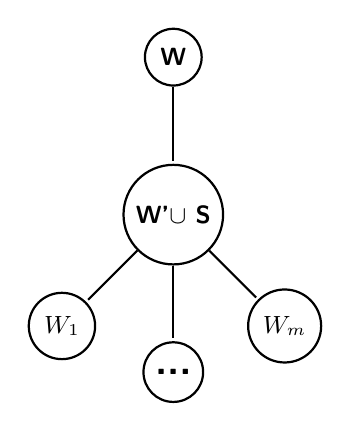
\begin{tikzpicture}[-,>=stealth',shorten >=1pt,auto,node distance=2.0cm,
  thick,main node/.style={circle,fill=white,draw,font=\sffamily\Large\bfseries}]

  \node[main node] (1) {\small{W}};
  \node[main node] (2) [below of=1]  {\small{W'$\cup$ S}};
  \node[main node] (3) [below left of=2] {\small{$W_{1}$}};
  \node[main node] (4) [below of=2]  {...};
  \node[main node] (5) [below right of=2] {\small{$W_{m}$}};
  
  \path[every node/.style={font=\sffamily\small}]
    (1) edge (2)
    (2) edge (3)
    (2) edge (4)
    (2) edge (5);
\end{tikzpicture}
\end{minipage}
\Else
\State {stop with output tw(G) $>$ k}
\EndIf
\EndProcedure
\end{algorithmic}
\end{algorithm}

\newpage

\subsubsection{Finding a nearly balanced W-seperator}

\begin{definition}
Let G be a graph and let W $\subseteq V(G)$. A nearly balanced separation of W is a triple (X, S, Y) where X, Y $\subseteq$ W and S $\subseteq V(G)$, such that \\

(1) W = $X \cup (S \cap W) \cup Y$ \\ 
(2) S seperates X and Y, and \\
(3) $0 < |X| < \frac{2}{3}|W|$ and $0 < |Y| < \frac{2}{3}|W|$.
\end{definition}

Instead of seperating X from Y, we seperate the neighbours of X from the neighbours of Y in $G \backslash (X \cup Y)$. The function disjoint\_ways, which implements a extended depth-first-search, computes a seperator of size at most k and aborts immediatly if no such seperator exists. 

\begin{algorithm}
\begin{algorithmic}[1]
\State {generate/enumerate all disjoint subsets of W of size 1 to 2$\cdot$k}
\For {all disjoint subsets X, Y of W}
\State {continue if there is an edge between vertices in X and Y in G}
\State {}
\State {Z := $W \backslash (X \cup Y)$}
\State {$S_{X}$ := $\{N_{G}(v): v \in X\} \cup Z$}
\State {$S_{Y}$ := $\{N_{G}(v): v \in Y\} \cup Z$}
\State {S := $S_{X} \cap S_{Y}$}
\State {H := $G \backslash (X \cup Y \cup S)$}
\State {$S_{X}$ := $S_{X} \backslash S$}
\State {$S_{Y}$ := $S_{Y} \backslash S$}
\State {}
\State {S := S $\cup$ disjoint\_ways(H, $S_{X}$, $S_{Y}$, k)}
\If {$|S|$ $>$ k+1 or $S \cap W$ != Z}
\State {continue}
\Else {}
\State {\Return S}
\EndIf
\EndFor
\State {\Return with output tw(G) $>$ k}
\end{algorithmic}
\end{algorithm}

For W $\subseteq V(G), |W| = 3k + 1$, a W-separation of order $\leq k + 1$, can be computed in time $O(3^{3k} \cdot k \cdot |E(G)|$. With this, we can, given a graph G as input, compute a tree decomposition width at most 4 $\cdot$ tw(G) + 1 in time $2^{O(k)}|V(G)|^{2}$. \\ 

\newpage

\subsubsection{Results}

\begin{table}[h!]
\begin{tabular}{|l|l|l|l|l|l|}
\hline
package & \#graphs & avg width & avg appr. & max width & time[ms] \\
\hline
\hline
stdlib & 142 & 5.85915 & 3.27934 & 8 & 676.673 \\
contiki & 1082 & 5.13771 & 3.18869 & 12 & 118254 \\
fuzix & 529 & 5.66541 & 3.04915 & 8 & 7390.37 \\
coremark & 42 & 5.59524 & 3.5119 & 8 & 392.223 \\
whetstone & 7 & 4.42857 & 3.35714 & 8 & 115.923 \\
dhrystone & 15 & 4.66667 & 2.93333 & 8 & 135.885 \\

\hline
\end{tabular}
\caption{Evaluation of the seperator-algorithm implementation. The worst approximation factor of 4 is adopted on almost each graph. The maximal width over all graphs, produced by the seperator algorithm was 8, graphs of higher treewidth could be decomposed with better approximation factor by tendency.}
\end{table}

\subsection{Usage}

\begin{lstlisting}[mathescape]
#include<tdlib/elimination_orderings.hpp>

graph_t G;
tree_dec_t T;

treedec::minDegree_decomp(G, T);
treedec::fillIn_decomp(G, T);

#include<tdlib/combinations.hpp>

treedec::PP_MD(G, T);
treedec::PP_FI(G, T);

#include<tdlib/separator_algorithm.hpp>

treedec::separator_algorithm(G, T);
\end{lstlisting}

\newpage

\section{Postprocessing}

\subsection{MinimumSeparatingVertexSets(MSVS)-heuristic}

\subsubsection{Algorithm}

The MinimumSeparatingVertexSets(MSVS)-heuristic \cite{B_tc1, Koster_thesis} tries to refine a maximum-sized bag with help of a seperator. For each pair of non-adjacent vertices there exists a seperator. To ensure the condition of connectivity on tree decomposition, the treated graphs - induced subgraphs of the current considered bag - are modified by inserting an edge if non-adjacent vertices occur in another bag in the current tree decomposition. If the modifiyed induced subgraph is not a complete graph, we can refine the current tree decomposition with respect to the considered bag by computing a seperator between a single pair of non-adjacent vertices or taking a minimal seperator, computed by considering all non-adjacent vertices and refine the tree decomposition with respect to the seperator as shown below.

\begin{algorithm}
$H_{i}$ denotes the graph with vertex set $X_{i}$ and edge set $\{\{j, k\}: j, k \in X_{i}\} \cup \{\{m, n\}: m, n \in X_{j} \cap X_{i}, j \neq i \}$ \\
\caption{MSVS-heuristic}
\begin{algorithmic}[1]
\While {$\exists i \in I$ such that $|X_{i}|$ maximal and $H_{i}$ does not induce a clique} 
\State {compute a minimum seperator $S \subset X_{i}$ in $H_{i}$}
\State {let $W_{i}$,...,$W_{r}$ define the r connected components of $H_{i}[X_{i} \backslash S]$}
\State {set I' = I \ \{i\} $\cup$ $\{i_{0},...,i_{r}\}$}
\State {set $X_{j}$' = $X_{j}$  $\forall j \neq i$, $X_{i_{0}}'$ = S, $X_{i_{q}}'$ = $W_{q} \cup S$  $\forall q \in \{1,...,r\}$}
\State {set F' = F $\backslash \{\{i, j\} \in N_{T}(i)\} \cup \{\{i_{0}, i_{q}\}: q = 1,...,r\} \cup \{\{j,i_{q}\}:j \in N_{T}(i)\}$ }
\State {   where $q_{j} \in \{1,...,r\}$ such that $X_{i} \cap X_{j} \subseteq W_{q_{i}} \cup S\}\}$}
\EndWhile
\end{algorithmic}
\begin{minipage}{0.2\textwidth}
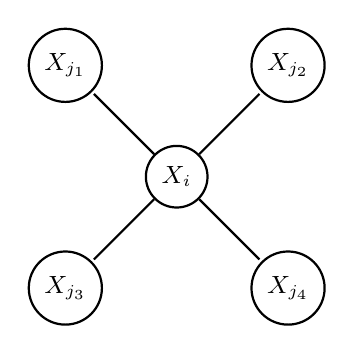
\begin{tikzpicture}[-,>=stealth',shorten >=1pt,auto,node distance=2.0cm,
  thick,main node/.style={circle,fill=white,draw,font=\sffamily\Large\bfseries}]

  \node[main node] (1) {\small{$X_{i}$}};
  \node[main node] (2) [above left of=1]  {\small{$X_{j_{1}}$}};
  \node[main node] (3) [above right of=1] {\small{$X_{j_{2}}$}};
  \node[main node] (4) [below left of=1]  {\small{$X_{j_{3}}$}};
  \node[main node] (5) [below right of=1] {\small{$X_{j_{4}}$}};
  
  \path[every node/.style={font=\sffamily\small}]
    (1) edge (2)
    (1) edge (3)
    (1) edge (4)
    (1) edge (5);
\end{tikzpicture}
\end{minipage}
\hspace{1.5cm}
\Huge{$\rightarrow$}
\normalsize
\begin{minipage}{0.2\textwidth}
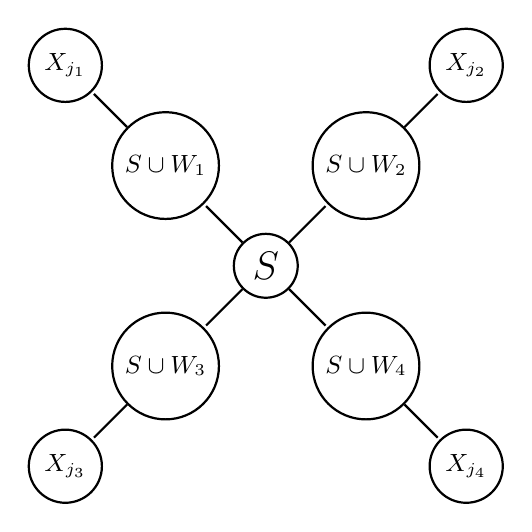
\begin{tikzpicture}[-,>=stealth',shorten >=1pt,auto,node distance=1.8cm,
  thick,main node/.style={circle,fill=white,draw,font=\sffamily\Large\bfseries}]

  \node[main node] (1) {$S$};
  \node[main node] (2) [above left of=1] {\small{$S \cup W_{1}$}};
  \node[main node] (3) [above right of=1] {\small{$S \cup W_{2}$}};
  \node[main node] (4) [below left of=1]  {\small{$S \cup W_{3}$}};
  \node[main node] (5) [below right of=1] {\small{$S \cup W_{4}$}};
  
  \node[main node] (6) [above left of=2]  {\small{$X_{j_{1}}$}};
  \node[main node] (7) [above right of=3] {\small{$X_{j_{2}}$}};
  \node[main node] (8) [below left of=4]  {\small{$X_{j_{3}}$}};
  \node[main node] (9) [below right of=5] {\small{$X_{j_{4}}$}};
  
  \path[every node/.style={font=\sffamily\small}]
    (1) edge (2)
    (1) edge (3)
    (1) edge (4)
    (1) edge (5)
    
    (2) edge (6)
    (3) edge (7)
    (4) edge (8)
    (5) edge (9);
\end{tikzpicture}
\end{minipage}
\end{algorithm}

\begin{comment}

%\subsubsection{Example}

In the following an example of how the MSVS-heuristic works is given. The input graph G is a 3x3-grid. On the left, the induced subgraph $H_{i}$ is shown, on the right the current tree decomposition, starting with a trivial one. The two blue-colored vertices are non-adjacent vertices, yellow-colored vertices show the computed seperating set, that seperates these non-adjacent vertices. red-colored edges are the edges in $E(H_{i}) \backslash E(G)$, that have to be added due to containment in other bags. Finally, the bag in the tree decomposition that will be improved has green color and the last computed seperator, that had become a bag is yellow-colored. \\ 

\vspace*{0.5cm}

\begin{minipage}{0.2\textwidth}
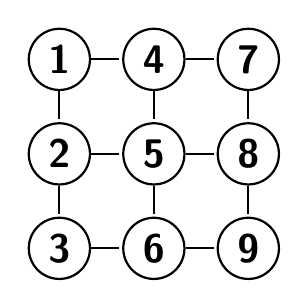
\begin{tikzpicture}[-,>=stealth',shorten >=1pt,auto,node distance=1.2cm,
  thick,main node/.style={circle,fill=white,draw,font=\sffamily\Large\bfseries},
        edge node/.style={circle,fill=purple,draw,font=\sffamily\Large\bfseries},
        sep node/.style={circle,fill=yellow,draw,font=\sffamily\Large\bfseries}]
  \node[main node] (1) {1};
  \node[main node] (2) [below of=1] {2};
  \node[main node] (3) [below of=2] {3};
  \node[main node] (4) [right of=1] {4};
  \node[main node] (5) [below of=4] {5};
  \node[main node] (6) [below of=5] {6};
  \node[main node] (7) [right of=4] {7};
  \node[main node] (8) [below of=7] {8};
  \node[main node] (9) [below of=8] {9};
  
  
  \path[every node/.style={font=\sffamily\small}]
    (1) edge (2)
    (1) edge (4)
    (2) edge (3)
    (2) edge (5)
    (3) edge (6)
    (4) edge (5)
    (4) edge (7)
    (5) edge (6)
    (5) edge (8)
    (6) edge (9)
    (7) edge (8)
    (8) edge (9);
\end{tikzpicture}
\end{minipage}
\hspace{3cm}
\begin{minipage}{0.2\textwidth}
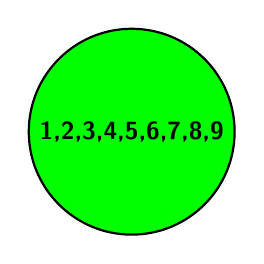
\begin{tikzpicture}[-,>=stealth',shorten >=1pt,auto,node distance=1.2cm,
  thick,main node/.style={circle,fill=white,draw,font=\sffamily\Large\bfseries},
  ref node/.style={circle,fill=green,draw,font=\sffamily\Large\bfseries}]
  \node[ref node] (1) {\small{1,2,3,4,5,6,7,8,9}};
\end{tikzpicture}
\end{minipage}

\vspace*{1cm}

\begin{minipage}{0.2\textwidth}
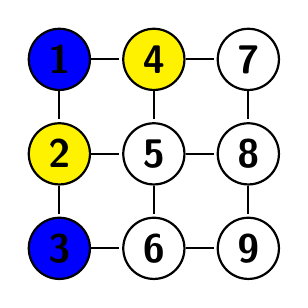
\begin{tikzpicture}[-,>=stealth',shorten >=1pt,auto,node distance=1.2cm,
  thick,main node/.style={circle,fill=white,draw,font=\sffamily\Large\bfseries},
        edge node/.style={circle,fill=blue,draw,font=\sffamily\Large\bfseries},
        sep node/.style={circle,fill=yellow,draw,font=\sffamily\Large\bfseries}]
  \node[edge node] (1) {1};
  \node[sep node]  (2) [below of=1] {2};
  \node[edge node] (3) [below of=2] {3};
  \node[sep node]  (4) [right of=1] {4};
  \node[main node] (5) [below of=4] {5};
  \node[main node] (6) [below of=5] {6};
  \node[main node] (7) [right of=4] {7};
  \node[main node] (8) [below of=7] {8};
  \node[main node] (9) [below of=8] {9};
  
  
  \path[every node/.style={font=\sffamily\small}]
    (1) edge (2)
    (1) edge (4)
    (2) edge (3)
    (2) edge (5)
    (3) edge (6)
    (4) edge (5)
    (4) edge (7)
    (5) edge (6)
    (5) edge (8)
    (6) edge (9)
    (7) edge (8)
    (8) edge (9);
\end{tikzpicture}
\end{minipage}
\hspace{3cm}
\begin{minipage}{0.2\textwidth}
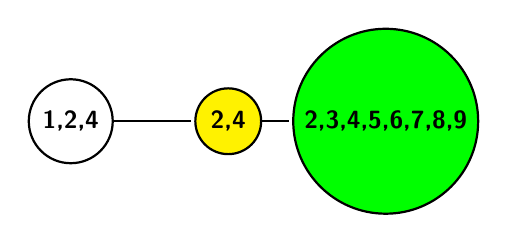
\begin{tikzpicture}[-,>=stealth',shorten >=1pt,auto,node distance=2cm,
  thick,main node/.style={circle,fill=white,draw,font=\sffamily\Large\bfseries},
  ref node/.style={circle,fill=green,draw,font=\sffamily\Large\bfseries},
  sep node/.style={circle,fill=yellow,draw,font=\sffamily\Large\bfseries}]
  \node[main node] (1) {\small{1,2,4}};
  \node[sep node]  (2) [right of=1] {\small{2,4}};
  \node[ref node]  (3) [right of=2] {\small{2,3,4,5,6,7,8,9}};
  
  \path[every node/.style={font=\sffamily\small}]
    (1) edge (2)
    (2) edge (3);
\end{tikzpicture}
\end{minipage}

\vspace*{1cm}

\begin{minipage}{0.2\textwidth}
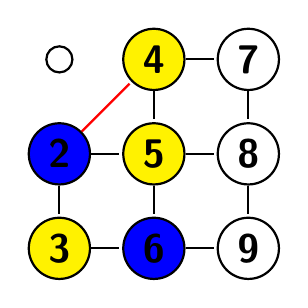
\begin{tikzpicture}[-,>=stealth',shorten >=1pt,auto,node distance=1.2cm,
  thick,main node/.style={circle,fill=white,draw,font=\sffamily\Large\bfseries},
        edge node/.style={circle,fill=blue,draw,font=\sffamily\Large\bfseries},
        sep node/.style={circle,fill=yellow,draw,font=\sffamily\Large\bfseries},
        inv node/.style={circle,draw,font=\sffamily\Large\bfseries}]
  \node[inv node]  (1) {};
  \node[edge node] (2) [below of=1] {2};
  \node[sep node]  (3) [below of=2] {3};
  \node[sep node]  (4) [right of=1] {4};
  \node[sep node] (5) [below of=4] {5};
  \node[edge node] (6) [below of=5] {6};
  \node[main node] (7) [right of=4] {7};
  \node[main node] (8) [below of=7] {8};
  \node[main node] (9) [below of=8] {9};
  
  
  \path[every node/.style={font=\sffamily\small}]
    (2) edge (3)
    (2) edge (5)
    (3) edge (6)
    (4) edge (5)
    (4) edge (7)
    (5) edge (6)
    (5) edge (8)
    (6) edge (9)
    (7) edge (8)
    (8) edge (9)
    (2) edge [draw=red] (4);
\end{tikzpicture} 
\end{minipage}
\hspace{3cm}
\begin{minipage}{0.2\textwidth}
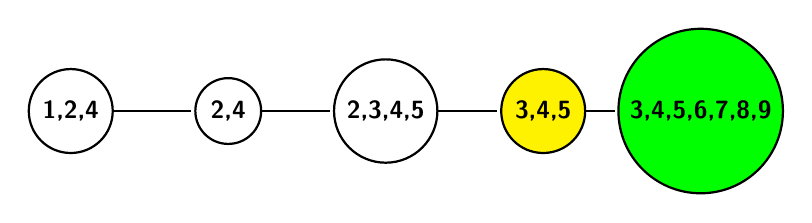
\begin{tikzpicture}[-,>=stealth',shorten >=1pt,auto,node distance=2cm,
  thick,main node/.style={circle,fill=white,draw,font=\sffamily\Large\bfseries},
  ref node/.style={circle,fill=green,draw,font=\sffamily\Large\bfseries},
  sep node/.style={circle,fill=yellow,draw,font=\sffamily\Large\bfseries}]
  \node[main node] (1) {\small{1,2,4}};
  \node[main node] (2) [right of=1] {\small{2,4}};
  \node[main node] (3) [right of=2] {\small{2,3,4,5}};
  \node[sep node]  (4) [right of=3] {\small{3,4,5}};
  \node[ref node]  (5) [right of=4] {\small{3,4,5,6,7,8,9}};
  
  \path[every node/.style={font=\sffamily\small}]
    (1) edge (2)
    (2) edge (3)
    (3) edge (4)
    (4) edge (5);
\end{tikzpicture}
\end{minipage}

\vspace*{1cm}

\begin{minipage}{0.2\textwidth}
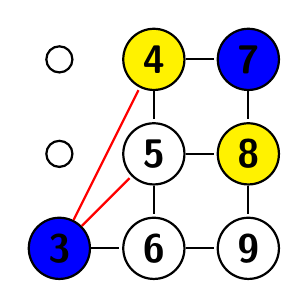
\begin{tikzpicture}[-,>=stealth',shorten >=1pt,auto,node distance=1.2cm,
  thick,main node/.style={circle,fill=white,draw,font=\sffamily\Large\bfseries},
        edge node/.style={circle,fill=blue,draw,font=\sffamily\Large\bfseries},
        sep node/.style={circle,fill=yellow,draw,font=\sffamily\Large\bfseries},
        inv node/.style={circle,draw,font=\sffamily\Large\bfseries}]
  \node[inv node]  (1) {};
  \node[inv node]  (2) [below of=1] {};
  \node[edge node] (3) [below of=2] {3};
  \node[sep node]  (4) [right of=1] {4};
  \node[main node] (5) [below of=4] {5};
  \node[main node] (6) [below of=5] {6};
  \node[edge node] (7) [right of=4] {7};
  \node[sep node]  (8) [below of=7] {8};
  \node[main node] (9) [below of=8] {9};
  
  
  \path[every node/.style={font=\sffamily\small}]
    (3) edge (6)
    (4) edge (5)
    (4) edge (7)
    (5) edge (6)
    (5) edge (8)
    (6) edge (9)
    (7) edge (8)
    (8) edge (9)
    (3) edge [draw=red] (4)
    (3) edge [draw=red] (5);
\end{tikzpicture}
\end{minipage}
\hspace{3cm}
\begin{minipage}{0.2\textwidth}
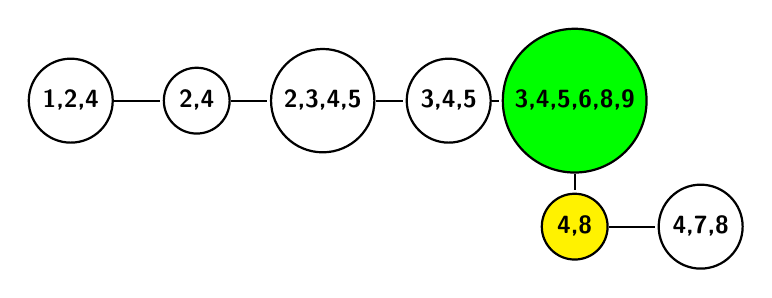
\begin{tikzpicture}[-,>=stealth',shorten >=1pt,auto,node distance=1.6cm,
  thick,main node/.style={circle,fill=white,draw,font=\sffamily\Large\bfseries},
  ref node/.style={circle,fill=green,draw,font=\sffamily\Large\bfseries},
  sep node/.style={circle,fill=yellow,draw,font=\sffamily\Large\bfseries}]
  \node[main node] (1) {\small{1,2,4}};
  \node[main node] (2) [right of=1] {\small{2,4}};
  \node[main node] (3) [right of=2] {\small{2,3,4,5}};
  \node[main node] (4) [right of=3] {\small{3,4,5}};
  \node[ref  node] (5) [right of=4] {\small{3,4,5,6,8,9}};
  \node[sep node]  (6) [below of=5] {\small{4,8}};
  \node[main node] (7) [right of=6] {\small{4,7,8}};
  
  \path[every node/.style={font=\sffamily\small}]
    (1) edge (2)
    (2) edge (3)
    (3) edge (4)
    (4) edge (5)
    (5) edge (6)
    (6) edge (7);
\end{tikzpicture}
\end{minipage}

\newpage

\begin{minipage}{0.2\textwidth}
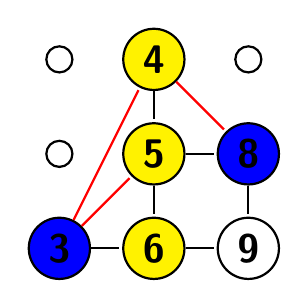
\begin{tikzpicture}[-,>=stealth',shorten >=1pt,auto,node distance=1.2cm,
  thick,main node/.style={circle,fill=white,draw,font=\sffamily\Large\bfseries},
        edge node/.style={circle,fill=blue,draw,font=\sffamily\Large\bfseries},
        sep node/.style={circle,fill=yellow,draw,font=\sffamily\Large\bfseries},
        inv node/.style={circle,draw,font=\sffamily\Large\bfseries}]
  \node[inv node]  (1) {};
  \node[inv node]  (2) [below of=1] {};
  \node[edge node] (3) [below of=2] {3};
  \node[sep node]  (4) [right of=1] {4};
  \node[sep node]  (5) [below of=4] {5};
  \node[sep node]  (6) [below of=5] {6};
  \node[inv node]  (7) [right of=4] {};
  \node[edge node] (8) [below of=7] {8};
  \node[main node] (9) [below of=8] {9};
  
  
  \path[every node/.style={font=\sffamily\small}]
    (3) edge (6)
    (4) edge (5)
    (5) edge (6)
    (5) edge (8)
    (6) edge (9)
    (8) edge (9)
    (3) edge [draw=red] (4)
    (3) edge [draw=red] (5)
    (4) edge [draw=red] (8);
\end{tikzpicture}
\end{minipage}
\hspace{3cm}
\begin{minipage}{0.2\textwidth}
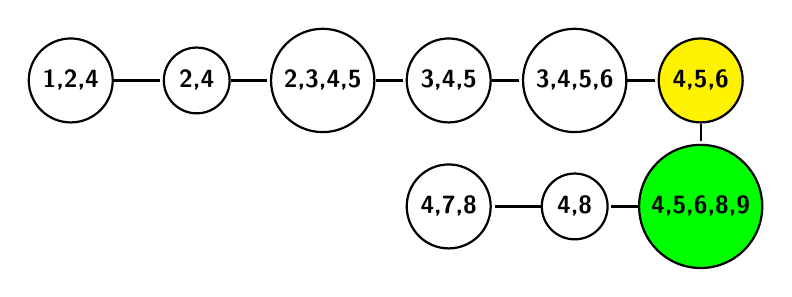
\begin{tikzpicture}[-,>=stealth',shorten >=1pt,auto,node distance=1.6cm,
  thick,main node/.style={circle,fill=white,draw,font=\sffamily\Large\bfseries},
  ref node/.style={circle,fill=green,draw,font=\sffamily\Large\bfseries},
  sep node/.style={circle,fill=yellow,draw,font=\sffamily\Large\bfseries}]
  \node[main node] (1) {\small{1,2,4}};
  \node[main node] (2) [right of=1] {\small{2,4}};
  \node[main node] (3) [right of=2] {\small{2,3,4,5}};
  \node[main node] (4) [right of=3] {\small{3,4,5}};
  \node[main node] (5) [right of=4] {\small{3,4,5,6}};
  \node[sep node]  (6) [right of=5] {\small{4,5,6}};
  \node[ref node]  (7) [below of=6] {\small{4,5,6,8,9}};
  \node[main node] (8) [left of=7] {\small{4,8}};
  \node[main node] (9) [left of=8] {\small{4,7,8}};
  
  \path[every node/.style={font=\sffamily\small}]
    (1) edge (2)
    (2) edge (3)
    (3) edge (4)
    (4) edge (5)
    (5) edge (6)
    (6) edge (7)
    (7) edge (8)
    (8) edge (9);
\end{tikzpicture}
\end{minipage}

\vspace*{1cm}

\begin{minipage}{0.2\textwidth}
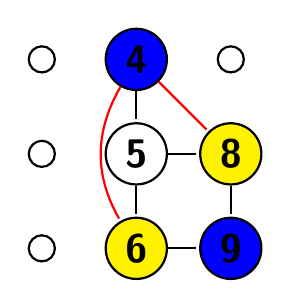
\begin{tikzpicture}[-,>=stealth',shorten >=1pt,auto,node distance=1.2cm,
  thick,main node/.style={circle,fill=white,draw,font=\sffamily\Large\bfseries},
        edge node/.style={circle,fill=blue,draw,font=\sffamily\Large\bfseries},
        sep node/.style={circle,fill=yellow,draw,font=\sffamily\Large\bfseries},
        inv node/.style={circle,draw,font=\sffamily\Large\bfseries}]
  \node[inv node]  (1) {};
  \node[inv node]  (2) [below of=1] {};
  \node[inv node]  (3) [below of=2] {};
  \node[edge node] (4) [right of=1] {4};
  \node[main node] (5) [below of=4] {5};
  \node[sep node]  (6) [below of=5] {6};
  \node[inv node]  (7) [right of=4] {};
  \node[sep node]  (8) [below of=7] {8};
  \node[edge node] (9) [below of=8] {9};
  
  
  \path[every node/.style={font=\sffamily\small}]
    (4) edge (5)
    (5) edge (6)
    (5) edge (8)
    (6) edge (9)
    (8) edge (9)
    (4) edge [draw=red, bend right] (6)
    (4) edge [draw=red] (8);
\end{tikzpicture}
\end{minipage}
\hspace{3cm}
\begin{minipage}{0.2\textwidth}
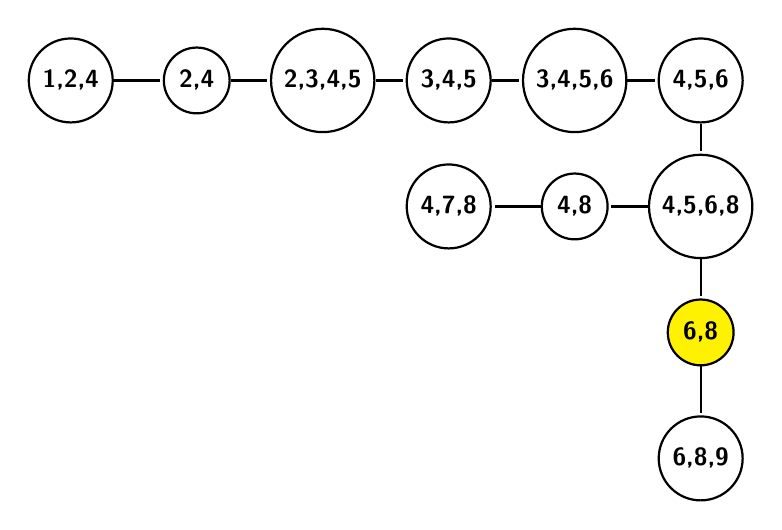
\begin{tikzpicture}[-,>=stealth',shorten >=1pt,auto,node distance=1.6cm,
  thick,main node/.style={circle,fill=white,draw,font=\sffamily\Large\bfseries},
  ref node/.style={circle,fill=green,draw,font=\sffamily\Large\bfseries},
  sep node/.style={circle,fill=yellow,draw,font=\sffamily\Large\bfseries}]
  \node[main node] (1) {\small{1,2,4}};
  \node[main node] (2) [right of=1] {\small{2,4}};
  \node[main node] (3) [right of=2] {\small{2,3,4,5}};
  \node[main node] (4) [right of=3] {\small{3,4,5}};
  \node[main node] (5) [right of=4] {\small{3,4,5,6}};
  \node[main node] (6) [right of=5] {\small{4,5,6}};
  \node[main node] (7) [below of=6] {\small{4,5,6,8}};
  \node[main node] (8) [left of=7] {\small{4,8}};
  \node[main node] (9) [left of=8] {\small{4,7,8}};
  \node[sep node]  (10) [below of=7] {\small{6,8}};
  \node[main node] (11) [below of=10] {\small{6,8,9}};
  
  \path[every node/.style={font=\sffamily\small}]
    (1) edge (2)
    (2) edge (3)
    (3) edge (4)
    (4) edge (5)
    (5) edge (6)
    (6) edge (7)
    (7) edge (8)
    (8) edge (9)
    (7) edge (10)
    (10) edge (11);
\end{tikzpicture}
\end{minipage}\\

We cannot proceed, because all bags of size 4 with additional edges induce a clique (e.g. $\{$4,5,6,7$\}$ with additional edges $\{$4,6$\}$, $\{$4,8$\}$ and $\{$6,8$\}$ induce a clique in G'. In this case, we obtained a tree decomposition of optimal width. \\

\end{comment}

\subsubsection{Results}

\begin{table}[h!]
\begin{tabular}{|l|l|l|l|l|}
\hline
package & \#graphs & avg width & max width & time[ms] \\
\hline
\hline
stdlib & 142 & 2.09859 & 6 & 744.505 \\
contiki & 1082 & 1.9085 & 10 & 9984.9 \\
fuzix & 529 & 2.26843 & 15 & 3171.12 \\
coremark & 42 & 2.07143 & 5 & 712.874 \\
whetstone & 7 & 1.57143 & 3 & 700.869 \\
dhrystone & 15 & 1.73333 & 3 & 984.715 \\

\hline
\end{tabular}
\caption{Results on applying MSVS on the trivial decomposition.}
\end{table}

\newpage

Results on applying MSVS on the tree decomposition returned by the seperator algorithm - this is a method to approximate the treewidth of a graph by a factor of 4 and hopefully reduce the bag size:

\begin{table}[h!]
\begin{tabular}{|l|l|l|l|l|l|}
\hline
package & \#graphs & avg width & max width & \#improved & time[ms] \\
\hline
\hline
stdlib & 142 & 4.59859 & 7 & 123 & 763.663 \\
contiki & 1082 & 3.7329 & 10 & 1010 & 124523 \\
fuzix & 529 & 4.31569 & 8 & 485 & 8331.65 \\
coremark & 42 & 4.28571 & 7 & 41 & 450.48 \\
whetstone & 7 & 3.42857 & 7 & 7 & 128.774 \\
dhrystone & 15 & 3.46667 & 7 & 14 & 135.773 \\

\hline
\end{tabular}

\caption{Applying the MSVS-heuristic on the treedecomposition, returned by the seperator algorithm. \#different denotes the count of graphs, where MSVS has reduced the width of the decomposition, that the seperator algorithm has computed.}
\end{table}

\subsection{Triangulation Minimization}

\subsubsection{LEX M}

The following algorithm returns a minimal ordering of a graph or a perfect ordering if the graph is chordal. Additionally, if the input graph is not chordal, the algorithm returns a set of edges, that are necessary to make the graph chordal:

\begin{algorithm}
\caption{LEX M}
\begin{algorithmic}[1]
\State {label(v) $\gets$ 0 $\forall v \in V(G)$}
\For {(i := $|V(G)|$; i $\geq$ 0; i$--$)}
\State {choose a unnumbered vertex v with label(v) = k}
\State {mark v reached}
\State {$\alpha$(i) := v}
\State {$\alpha ^{-1}$(v) := i}
\State {reach(j) $\gets \emptyset$ $\forall j \in \{$1, .., k$\}$}
\State {mark all unnumbered vertices unreached}
\For {w $\in N_{G}(v)$ and $\alpha ^{-1}$(w) = 0}
\State {add w to reach(label(w))}
\State {mark w reached}
\State {label(w) += 0.5}
\State {add an edge $\{v, w\}$ to $G^{+}$}
\EndFor
\For {(j := 1; j $\leq$ k; j++)}
\While {reach(j) $\neq \emptyset$}
\State {delete a vertex w from reach(j)}
\For {z $\in N_{G}(w)$ and z unreached}
\State {mark z reached}
\If {label(z) $>$ j}
\State {add z to reach(label(z))}
\State {label(z) := label(z) + 0.5}
\State {add an edge $\{v, z\}$ to $G^{+}$}
\Else { add z to reach(j)}
\EndIf
\EndFor
\EndWhile
\EndFor
\State {sort unnumbered vertices by label(w) value (radix-sort)}
\State {redefine k}
\State {reassign label(w) values to be integers from 1 to k}
\EndFor
\end{algorithmic}
\end{algorithm}

\newpage

\begin{comment}

\underline{\textbf{Example}}

\vspace*{0.1cm}

\begin{minipage}{0.2\textwidth}
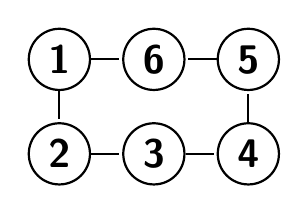
\begin{tikzpicture}[-,>=stealth',shorten >=1pt,auto,node distance=1.2cm,
  thick,main node/.style={circle,fill=white,draw,font=\sffamily\Large\bfseries},
        edge node/.style={circle,fill=purple,draw,font=\sffamily\Large\bfseries},
        sep node/.style={circle,fill=yellow,draw,font=\sffamily\Large\bfseries}]
  \node[main node] (1) {1};
  \node[main node] (2) [below of=1] {2};
  \node[main node] (3) [right of=2] {3};
  \node[main node] (4) [right of=3] {4};
  \node[main node] (5) [above of=4] {5};
  \node[main node] (6) [right of=1] {6};  
  
  \path[every node/.style={font=\sffamily\small}]
    (1) edge (2)
    (1) edge (6)
    (2) edge (3)
    (3) edge (4)
    (4) edge (5)
    (5) edge (6);
\end{tikzpicture}
\end{minipage}
\hspace{3cm}
\begin{minipage}{0.5\textwidth}
\begin{tabular}{l|l|l|l|l|l|l}
\small
label & $v_{1}$ & $v_{2}$ & $v_{3}$ & $v_{4}$ & $v_{5}$ & $v_{6}$ \\
\hline
      & 1       & 1       & 1       & 1       & 1       & 1       \\
\end{tabular} \\
k = 1 \\
v := $v_{1}$ \\
w = $v_{2}$, $v_{6}$ \\
label($v_{2}$), label($v_{6}$) += 0.5 \\
there is no unvisited vertex z, such that label(z) $>$ 1 \\
\end{minipage}

\vspace*{0.3cm}

\begin{minipage}{0.2\textwidth}
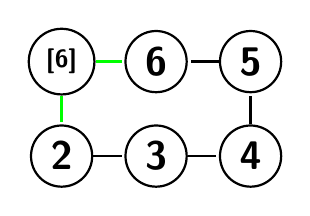
\begin{tikzpicture}[-,>=stealth',shorten >=1pt,auto,node distance=1.2cm,
  thick,main node/.style={circle,fill=white,draw,font=\sffamily\Large\bfseries},
        edge node/.style={circle,fill=purple,draw,font=\sffamily\Large\bfseries},
        sep node/.style={circle,fill=yellow,draw,font=\sffamily\Large\bfseries}]
  \node[main node] (1) {\small [6]};
  \node[main node] (2) [below of=1] {2};
  \node[main node] (3) [right of=2] {3};
  \node[main node] (4) [right of=3] {4};
  \node[main node] (5) [above of=4] {5};
  \node[main node] (6) [right of=1] {6};  
  
  \path[every node/.style={font=\sffamily\small}]
    (1) edge [draw=green] (2)
    (1) edge [draw=green] (6)
    (2) edge (3)
    (3) edge (4)
    (4) edge (5)
    (5) edge (6);
\end{tikzpicture}
\end{minipage}
\hspace{3cm}
\begin{minipage}{0.5\textwidth}
\begin{tabular}{l|l|l|l|l|l|l}
\small
label & $v_{1}$ & $v_{2}$ & $v_{3}$ & $v_{4}$ & $v_{5}$ & $v_{6}$ \\
\hline
      & 1       & 2       & 1       & 1       & 1       & 2       \\
\end{tabular} \\
k = 2 \\
v := $v_{2}$ \\
w = $v_{3}$  \\
label($v_{3}$) += 0.5 \\
the path $v_{3}$, $v_{4}$, $v_{5}$, $v_{6}$ fulfills the condition $\rightarrow$ add $\{v_{2}$, $v_{6}\}$ to $G^{+}$ \\
\end{minipage}

\vspace*{0.3cm}

\begin{minipage}{0.2\textwidth}
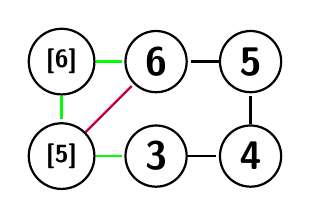
\begin{tikzpicture}[-,>=stealth',shorten >=1pt,auto,node distance=1.2cm,
  thick,main node/.style={circle,fill=white,draw,font=\sffamily\Large\bfseries},
        edge node/.style={circle,fill=purple,draw,font=\sffamily\Large\bfseries},
        sep node/.style={circle,fill=yellow,draw,font=\sffamily\Large\bfseries}]
  \node[main node] (1) {\small [6]};
  \node[main node] (2) [below of=1] {\small [5]};
  \node[main node] (3) [right of=2] {3};
  \node[main node] (4) [right of=3] {4};
  \node[main node] (5) [above of=4] {5};
  \node[main node] (6) [right of=1] {6};  
  
  \path[every node/.style={font=\sffamily\small}]
    (1) edge [draw=green] (2)
    (1) edge [draw=green] (6)
    (2) edge [draw=green] (3)
    (3) edge (4)
    (4) edge (5)
    (5) edge (6)
    
    (2) edge [draw=purple] (6);
\end{tikzpicture}
\end{minipage}
\hspace{3cm}
\begin{minipage}{0.5\textwidth}
\begin{tabular}{l|l|l|l|l|l|l}
\small
label & $v_{1}$ & $v_{2}$ & $v_{3}$ & $v_{4}$ & $v_{5}$ & $v_{6}$ \\
\hline
      & 1       & 2       & 2       & 1       & 1       & 3       \\
\end{tabular} \\
k = 3 \\
v := $v_{6}$ \\
w = $v_{5}$  \\
label($v_{5}$) += 0.5 \\
the path $v_{5}$, $v_{4}$, $v_{3}$ fulfills the condition $\rightarrow$ add $\{v_{6}$, $v_{3}\}$ to $G^{+}$ \\
\end{minipage}

\vspace*{0.3cm}

\begin{minipage}{0.2\textwidth}
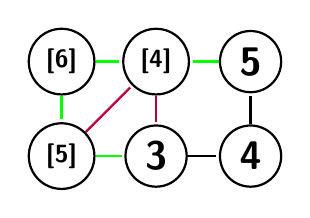
\begin{tikzpicture}[-,>=stealth',shorten >=1pt,auto,node distance=1.2cm,
  thick,main node/.style={circle,fill=white,draw,font=\sffamily\Large\bfseries},
        edge node/.style={circle,fill=purple,draw,font=\sffamily\Large\bfseries},
        sep node/.style={circle,fill=yellow,draw,font=\sffamily\Large\bfseries}]
  \node[main node] (1) {\small[6]};
  \node[main node] (2) [below of=1] {\small[5]};
  \node[main node] (3) [right of=2] {3};
  \node[main node] (4) [right of=3] {4};
  \node[main node] (5) [above of=4] {5};
  \node[main node] (6) [right of=1] {\small[4]};  
  
  \path[every node/.style={font=\sffamily\small}]
    (1) edge [draw=green] (2)
    (1) edge [draw=green] (6)
    (2) edge [draw=green](3)
    (3) edge (4)
    (4) edge (5)
    (5) edge [draw=green] (6)
    
    (2) edge [draw=purple] (6)
    (6) edge [draw=purple] (3);
\end{tikzpicture}
\end{minipage}
\hspace{3cm}
\begin{minipage}{0.5\textwidth}
\begin{tabular}{l|l|l|l|l|l|l}
\small
label & $v_{1}$ & $v_{2}$ & $v_{3}$ & $v_{4}$ & $v_{5}$ & $v_{6}$ \\
\hline
      & 1       & 2       & 3       & 1       & 2       & 3       \\
\end{tabular} \\
k = 3 \\
v := $v_{3}$ \\
w = $v_{4}$  \\
label($v_{4}$) += 0.5 \\
the path $v_{4}$, $v_{5}$ fulfills the condition $\rightarrow$ add $\{v_{3}$, $v_{5}\}$ to $G^{+}$ \\
\end{minipage}

\vspace*{0.3cm}

\begin{minipage}{0.2\textwidth}
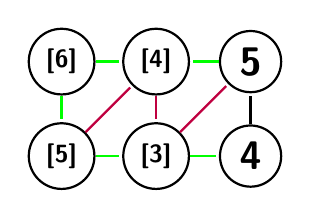
\begin{tikzpicture}[-,>=stealth',shorten >=1pt,auto,node distance=1.2cm,
  thick,main node/.style={circle,fill=white,draw,font=\sffamily\Large\bfseries},
        edge node/.style={circle,fill=purple,draw,font=\sffamily\Large\bfseries},
        sep node/.style={circle,fill=yellow,draw,font=\sffamily\Large\bfseries}]
  \node[main node] (1) {\small [6]};
  \node[main node] (2) [below of=1] {\small [5]};
  \node[main node] (3) [right of=2] {\small [3]};
  \node[main node] (4) [right of=3] {4};
  \node[main node] (5) [above of=4] {5};
  \node[main node] (6) [right of=1] {\small [4]};  
  
  \path[every node/.style={font=\sffamily\small}]
    (1) edge [draw=green] (2)
    (1) edge [draw=green] (6)
    (2) edge [draw=green] (3)
    (3) edge [draw=green] (4)
    (4) edge (5)
    (5) edge [draw=green] (6)
    
    (2) edge [draw=purple] (6)
    (6) edge [draw=purple] (3)
    (3) edge [draw=purple] (5);
\end{tikzpicture}
\end{minipage}
\hspace{3cm}
\begin{minipage}{0.5\textwidth}
\begin{tabular}{l|l|l|l|l|l|l}
\small
label & $v_{1}$ & $v_{2}$ & $v_{3}$ & $v_{4}$ & $v_{5}$ & $v_{6}$ \\
\hline
      & 1       & 2       & 3       & 2       & 3       & 3       \\
\end{tabular} \\
k = 3 \\
v := $v_{5}$ \\
w = $v_{4}$  \\
label($v_{4}$) += 0.5 \\
\end{minipage}

\newpage

\begin{minipage}{0.2\textwidth}
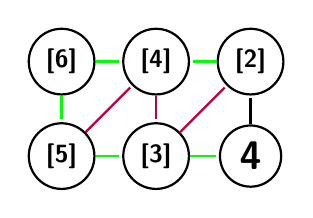
\begin{tikzpicture}[-,>=stealth',shorten >=1pt,auto,node distance=1.2cm,
  thick,main node/.style={circle,fill=white,draw,font=\sffamily\Large\bfseries},
        edge node/.style={circle,fill=purple,draw,font=\sffamily\Large\bfseries},
        sep node/.style={circle,fill=yellow,draw,font=\sffamily\Large\bfseries}]
  \node[main node] (1) {\small [6]};
  \node[main node] (2) [below of=1] {\small [5]};
  \node[main node] (3) [right of=2] {\small [3]};
  \node[main node] (4) [right of=3] {4};
  \node[main node] (5) [above of=4] {\small [2]};
  \node[main node] (6) [right of=1] {\small [4]};  
  
  \path[every node/.style={font=\sffamily\small}]
    (1) edge [draw=green] (2)
    (1) edge [draw=green] (6)
    (2) edge [draw=green] (3)
    (3) edge [draw=green] (4)
    (4) edge (5)
    (5) edge [draw=green] (6)
    
    (2) edge [draw=purple] (6)
    (6) edge [draw=purple] (3)
    (3) edge [draw=purple] (5);
\end{tikzpicture}
\end{minipage}
\hspace{3cm}
\begin{minipage}{0.2\textwidth}
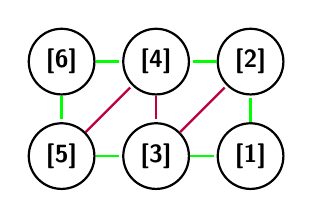
\begin{tikzpicture}[-,>=stealth',shorten >=1pt,auto,node distance=1.2cm,
  thick,main node/.style={circle,fill=white,draw,font=\sffamily\Large\bfseries},
        edge node/.style={circle,fill=purple,draw,font=\sffamily\Large\bfseries},
        sep node/.style={circle,fill=yellow,draw,font=\sffamily\Large\bfseries}]
  \node[main node] (1) {\small [6]};
  \node[main node] (2) [below of=1] {\small [5]};
  \node[main node] (3) [right of=2] {\small [3]};
  \node[main node] (4) [right of=3] {\small [1]};
  \node[main node] (5) [above of=4] {\small [2]};
  \node[main node] (6) [right of=1] {\small [4]};  
  
  \path[every node/.style={font=\sffamily\small}]
    (1) edge [draw=green] (2)
    (1) edge [draw=green] (6)
    (2) edge [draw=green] (3)
    (3) edge [draw=green] (4)
    (4) edge [draw=green] (5)
    (5) edge [draw=green] (6)
    
    (2) edge [draw=purple] (6)
    (6) edge [draw=purple] (3)
    (3) edge [draw=purple] (5);
\end{tikzpicture}
\end{minipage}

\vspace*{0.5cm}

Since all vertices have been numbered, we are done. If we eliminate the vertices in the given ordering on the original graph, the purple-colored vertices will be added as fill-in edges: they are necessary edges in a triangulation of the input graph. \\

\end{comment}

\subsubsection{MinimalChordal}

\begin{definition}
Let $G^{+}$ be a chordal supergraph of a graph G. A \textbf{candidate edge} is an edge $uv \in E(G^{+})\backslash E(G)$ which is not the unique chord of any 4-cycle in $G^{+}$.
\end{definition}

A non-minimal chordal supergraph $G^{+}$ of a graph G with respect to elimination ordering $\alpha$ has at least one candidate edge. Any candidate edge can be removed without destroying chordality. If we have a minimal chordal supergraph $G'^{+}$ of G that results after removing all candidate edge, we can compute a perfect elimination ordering $\beta$, that may cause lower width of a tree decomposition in comparision to $\alpha$ when applied to G. \\

The following algorithm assumes that the graph containing the neighbourhood after eliminating a vertex in step i in the elimination game is stored in $C_{i}$ and the edges added in this step are stored in $F_{i}$. This can be done while computing the fill-in graph of the input graph in step 1. After this, we check for $i = |V(G)|, \dots, 1$ if any candidate edge is contained in $F_{i}$. If this is the case, we run LEX-M on the graph without the candidate edges to find out, which edges are necessary in a triangulation of the input graph. Candidate edges, that are not necessary according to LEX-M can be removed in the fill-in graph.
After doing these steps in all iterations, we can construct - the modified fill-in graph is still chordal - a different perfect elimination ordering of this one using the LEX-P algorithm.

\begin{algorithm}
\caption{MinimalChordal}
\begin{algorithmic}[1]
\State {M $\gets$ fill-in graph of G with respect to $\alpha$}
\For {i := $|V(G)|$; i $\geq$ 1; i$--$)}
\State {Candidate(i) = $\emptyset$}
\State {Incident(i) = $\emptyset$}
\For {all $\{u, v\} \in F_{i}$}
\If {is\_candidate\_edge($\{u, v\}$, i, M)}
\State {Candidate(i) = Candidate(i) $\cup$ $\{\{u, v\}\}$}
\State {Incident(i) = Incident(i) $\cup$ $\{u, v\}$}
\EndIf
\EndFor
\If {Candidate(i) $\neq \emptyset$}
\State {$W_{i} = C_{i}$[Incident(i)] $\backslash$ Candidate(i)}
\State {KeepFill(i) = $LEX-M(W_{i})$}
\State {E(M) = E(M) $\backslash$ (Candidate(i) $\backslash$ KeepFill(i))}
\EndIf
\EndFor
\State {\Return {M and $\beta = LEX-P(M)$}}
\end{algorithmic}
\end{algorithm}

\newpage

\subsubsection{Results}

Triangulation minimization has no effect on tree decomposition returned from the minDegree-heuristic, but reduces the width for some tree decompositions returned by the fillIn-heuristic:

\begin{table}[h!]
\underline{\textbf{fillIn-heuristic + triangulation minimization}} \\
\begin{tabular}{|l|l|l|l|l|l|}
\hline
package & \#graphs & avg width & max width & max width & time[ms] \\
\hline
\hline
stdlib & 142 & 1.85211 & 4 & 2 & 91.67 \\
contiki & 1082 & 1.71349 & 7 & 14 & 873.177 \\
fuzix & 529 & 1.96597 & 6 & 14 & 388.394 \\
coremark & 42 & 1.64286 & 3 & 2 & 77.216 \\
whetstone & 7 & 1.42857 & 2 & 0 & 27.616 \\
dhrystone & 15 & 1.66667 & 2 & 0 & 37.236 \\

\hline
\end{tabular}
\end{table}

\begin{table}[h!]
\underline{\textbf{preprocessing + fillIn-heuristic + triangulation minimization}} \\
\begin{tabular}{|l|l|l|l|l|l|}
\hline
package & \#graphs & avg width & max width & \#improved & time[ms] \\
\hline
\hline
stdlib & 142 & 1.85211 & 4 & 0 & 25.914 \\
contiki & 1082 & 1.71165 & 7 & 0 & 348.045 \\
fuzix & 529 & 1.96597 & 6 & 0 & 133.571 \\
coremark & 42 & 1.64286 & 3 & 0 & 14.508 \\
whetstone & 7 & 1.42857 & 2 & 0 & 3.84 \\
dhrystone & 15 & 1.66667 & 2 & 0 & 4.685 \\

\hline
\end{tabular}
\end{table}

\begin{table}[h!]
\underline{\textbf{seperator algorithm + triangulation minimization}} \\
\begin{tabular}{|l|l|l|l|l|l|}
\hline
package & \#graphs & avg width & max width & \#improved & time[ms] \\
\hline
\hline
stdlib & 142 & 2.11972 & 6 & 142 & 760.169 \\
contiki & 1082 & 1.89002 & 9 & 1070 & 124127 \\
fuzix & 529 & 2.21172 & 7 & 525 & 7781.26 \\
coremark & 42 & 2.02381 & 6 & 42 & 454.19 \\
whetstone & 7 & 1.57143 & 3 & 7 & 139.376 \\
dhrystone & 15 & 1.73333 & 3 & 15 & 162.553 \\

\hline
\end{tabular}
\caption{Applying the minimalChordal-heuristic on the treedecomposition returned by the seperator algorithm.}
\end{table}

\newpage

\section{Applications}

In this section, we give an overview about the implemented algorithms, that solve hard problems based on tree decompositions. Until now, we implemented algorithms for the following problems.

\begin{itemize}
\item max-Clique
\item min-Vertex Cover
\item max-Independent Set
\item min-Dominating Set
\item min-Colorability
\end{itemize}

Except for the max-Clique problem, the algorithms work only on nice tree decompositions. 

\begin{comment}

%\subsection{max-Clique}

max-Clique is computed by solving max-Clique on the by bags induced subgraphs of the input graph for all bags of the tree decomposition. The answer is the maximum size of a clique, that has been computed in this way. This is the case, because clique must be fully contained in some bag of a tree decomposition. The algorithm works in time $\mathcal{|V(G)| \cdot 2^{\operatorname{tw}(G)+1}}$. If the input graph has small treewidth, e.g. k is a small constant, the algorithms work in linear time. 

\end{comment}

%\subsection{min-Vertex Cover} 

\subsection{Results}

\underline{\textbf{max-Clique}} \\
\begin{tabular}{|l|l|l|l|l|l|l|l|l|}
\hline
package & \#graphs & avg width & max width & time1[ms] & avg set size & max set size & time2[ms] & totaltime \\
\hline
\hline
stdlib & 142 & 1.85211 & 4 & 14.182 & 2.09155 & 3 & 2.892 & 17.074 \\
contiki & 1082 & 1.72089 & 8 & 107.673 & 2.08595 & 3 & 23.73 & 131.403 \\
fuzix & 529 & 1.96975 & 6 & 61.131 & 2.16068 & 3 & 13.019 & 74.15 \\
coremark & 42 & 1.64286 & 3 & 6.235 & 2.11905 & 3 & 0.992 & 7.227 \\
whetstone & 7 & 1.42857 & 2 & 1.687 & 2 & 2 & 0.476 & 2.163 \\
dhrystone & 15 & 1.66667 & 2 & 2.102 & 2.13333 & 3 & 0.529 & 2.631 \\

\hline
\end{tabular}

\vspace*{5mm}

\underline{\textbf{max-Independent Set}} \\
\begin{tabular}{|l|l|l|l|l|l|l|l|l|}
\hline
package & \#graphs & avg width & max width & time1[ms] & avg set size & max set size & time2[ms] & totaltime \\
\hline
\hline
stdlib & 142 & 1.85211 & 4 & 14.198 & 18.9155 & 275 & 102.011 & 116.209 \\
contiki & 1082 & 1.72089 & 8 & 108.931 & 18.4381 & 724 & 999.048 & 1107.98 \\
fuzix & 529 & 1.96975 & 6 & 62.569 & 21.2684 & 292 & 557.929 & 620.498 \\
coremark & 42 & 1.64286 & 3 & 6.666 & 28.381 & 316 & 55.363 & 62.029 \\
whetstone & 7 & 1.42857 & 2 & 1.837 & 45.1429 & 228 & 15.142 & 16.979 \\
dhrystone & 15 & 1.66667 & 2 & 2.838 & 28 & 267 & 21.43 & 24.268 \\

\hline
\end{tabular}

\vspace*{5mm}

\underline{\textbf{min-Vertex Cover}} \\
\begin{tabular}{|l|l|l|l|l|l|l|l|l|}
\hline
package & \#graphs & avg width & max width & time1[ms] & avg set size & max set size & time2[ms] & totaltime \\
\hline
\hline
stdlib & 142 & 1.85211 & 4 & 14.275 & 18.5563 & 269 & 117.755 & 132.03 \\
contiki & 1082 & 1.72089 & 8 & 107.858 & 18.0564 & 728 & 1113.7 & 1221.56 \\
fuzix & 529 & 1.96975 & 6 & 62.744 & 20.7221 & 295 & 636.881 & 699.625 \\
coremark & 42 & 1.64286 & 3 & 6.383 & 27.881 & 321 & 55.287 & 61.67 \\
whetstone & 7 & 1.42857 & 2 & 1.687 & 44 & 225 & 14.586 & 16.273 \\
dhrystone & 15 & 1.66667 & 2 & 2.16 & 27.4 & 267 & 18.626 & 20.786 \\

\hline
\end{tabular}

\newpage

\underline{\textbf{min-Dominating Set}} \\
\begin{tabular}{|l|l|l|l|l|l|l|l|l|}
\hline
package & \#graphs & avg width & max width & time1[ms] & avg set size & max set size & time2[ms] & totaltime \\
\hline
\hline
\input{./Results/26_min_dominating_set.tex}
\hline
\end{tabular}

\vspace*{5mm}

\underline{\textbf{min-Colorabilty}} \\
\begin{tabular}{|l|l|l|l|l|l|l|l|l|}
\hline
package & \#graphs & avg width & max width & time1[ms] & avg set size & max set size & time2[ms] & totaltime \\
\hline
\hline
stdlib & 142 & 1.85211 & 4 & 14.562 & 2.59155 & 3 & 293.238 & 307.8 \\
contiki & 1082 & 1.72089 & 8 & 111.881 & 2.42144 & 3 & 203687 & 203799 \\
fuzix & 529 & 1.96975 & 6 & 65.619 & 2.51796 & 3 & 5663.1 & 5728.72 \\
coremark & 42 & 1.64286 & 3 & 6.605 & 2.47619 & 3 & 174.581 & 181.186 \\
whetstone & 7 & 1.42857 & 2 & 1.66 & 2.14286 & 3 & 70.074 & 71.734 \\
dhrystone & 15 & 1.66667 & 2 & 2.125 & 2.33333 & 3 & 81.407 & 83.532 \\

\hline
\end{tabular}

\subsection{Usage}

\begin{lstlisting}[mathescape]
#include<tdlib/combinations.hpp>
#include<tdlib/nice_decomposition.hpp>
#include<tdlib/applications.hpp>
#include<tdlib/misc.hpp>

graph_t G;
graph_t H;
tree_dec_t T;

H = G;

treedec::PP_MD(G, T);

tree_dec_dir_t T2;

treedec::make_rooted(T, T2);
treedec::nice::nicify(T2);

std::set<unsigned int> S;
unsigned k =
  treedec::app::max_clique_with_treedecomposition(H, T2, S);
unsigned k =
  treedec::app::max_independent_set_with_treedecomposition(H, T2, S);
unsigned k = 
  treedec::app::min_vertex_cover_with_treedecomposition(H, T2, S);
unsigned k =
  treedec::app::min_dominating_set_with_treedecomposition(H, T2, S);

std::vector<std::set<unsigned int> > S;
unsigned k =
  treedec::app::min_coloring_with_treedecomposition(H, T2, S);
\end{lstlisting}

\newpage

\section{pytdlib}

./configue --with-python=python2.7 or ./configure --with-python=python3.x \\

make install; python; import tdlib; help(tdlib);

\newpage

\section{Summary}

\subsection{Comparison of the algorithms}

\vspace*{0.5cm}

\oddsidemargin0pt
\textheight700pt

\begin{minipage}{0.2\textwidth}
\underline{\textbf{Seperator algorithm}} \\
\small{
\begin{tabular}{|l|l|l|l|l|}
\hline
package & \#graphs & avg width & max width & time[ms] \\
\hline
\hline
stdlib & 142 & 5.85915 & 8 & 678.271 \\
contiki & 1082 & 5.13771 & 12 & 120944 \\
fuzix & 529 & 5.66541 & 8 & 7405.06 \\
coremark & 42 & 5.59524 & 8 & 390.035 \\
whetstone & 7 & 4.42857 & 8 & 118.97 \\
dhrystone & 15 & 4.66667 & 8 & 128.536 \\

\hline
\end{tabular}
}
\end{minipage}
\hspace{6.5cm}
\begin{minipage}{0.2\textwidth}
\underline{\textbf{MSVS trivial}} \\
\small{
\begin{tabular}{|l|l|l|l|l|}
\hline
package & \#graphs & avg width & max width & time[ms] \\
\hline
\hline
stdlib & 142 & 2.09859 & 6 & 744.505 \\
contiki & 1082 & 1.9085 & 10 & 9984.9 \\
fuzix & 529 & 2.26843 & 15 & 3171.12 \\
coremark & 42 & 2.07143 & 5 & 712.874 \\
whetstone & 7 & 1.57143 & 3 & 700.869 \\
dhrystone & 15 & 1.73333 & 3 & 984.715 \\

\hline
\end{tabular}
}
\end{minipage}

\vspace*{0.5cm}

\begin{minipage}{0.2\textwidth}
\underline{\textbf{Seperator algorithm + MSVS}} \\
\small{
\begin{tabular}{|l|l|l|l|l|}
\hline
package & \#graphs & avg width & max width & time[ms] \\
\hline
\hline
stdlib & 142 & 4.59859 & 7 & 817.434 \\
contiki & 1082 & 3.7329 & 10 & 120149 \\
fuzix & 529 & 4.31569 & 8 & 7697.91 \\
coremark & 42 & 4.28571 & 7 & 463.817 \\
whetstone & 7 & 3.42857 & 7 & 163.421 \\
dhrystone & 15 & 3.46667 & 7 & 134.822 \\

\hline
\end{tabular}
}
\end{minipage}
\hspace{6.5cm}
\begin{minipage}{0.2\textwidth}
\underline{\textbf{Seperator algorithm + TM}} \\
\small{
\begin{tabular}{|l|l|l|l|l|}
\hline
package & \#graphs & avg width & max width & time[ms] \\
\hline
\hline
stdlib & 142 & 2.11972 & 6 & 752.575 \\
contiki & 1082 & 1.89002 & 9 & 121920 \\
fuzix & 529 & 2.21172 & 7 & 7689.25 \\
coremark & 42 & 2.02381 & 6 & 448.473 \\
whetstone & 7 & 1.57143 & 3 & 130.814 \\
dhrystone & 15 & 1.73333 & 3 & 154.16 \\

\hline
\end{tabular}
}
\end{minipage}

\vspace*{0.5cm}

\begin{minipage}{0.2\textwidth}
\underline{\textbf{minDegree-heuristic}} \\
\small{
\begin{tabular}{|l|l|l|l|l|}
\hline
package & \#graphs & avg width & max width & time[ms] \\
\hline
\hline
stdlib & 142 & 1.85211 & 4 & 14.439 \\
contiki & 1082 & 1.72089 & 8 & 112.864 \\
fuzix & 529 & 1.96975 & 6 & 60.839 \\
coremark & 42 & 1.64286 & 3 & 6.219 \\
whetstone & 7 & 1.42857 & 2 & 1.647 \\
dhrystone & 15 & 1.66667 & 2 & 2.143 \\

\hline
\end{tabular}
}
\end{minipage}
\hspace{6.5cm}
\begin{minipage}{0.2\textwidth}
\underline{\textbf{preprocessing + minDegree-heuristic}} \\
\small{
\begin{tabular}{|l|l|l|l|l|}
\hline
package & \#graphs & avg width & max width & time[ms] \\
\hline
\hline
stdlib & 142 & 1.85211 & 4 & 24.23 \\
contiki & 1082 & 1.71442 & 7 & 286.349 \\
fuzix & 529 & 1.96597 & 6 & 119.968 \\
coremark & 42 & 1.64286 & 3 & 17.483 \\
whetstone & 7 & 1.42857 & 2 & 6.185 \\
dhrystone & 15 & 1.66667 & 2 & 4.643 \\

\hline
\end{tabular}
}
\end{minipage}

\vspace*{0.5cm}

\begin{minipage}{0.2\textwidth}
\underline{\textbf{minFill-heuristic}} \\
\small{
\begin{tabular}{|l|l|l|l|l|}
\hline
package & \#graphs & avg width & max width & time[ms] \\
\hline
\hline
stdlib & 142 & 1.8662 & 4 & 19.401 \\
contiki & 1082 & 1.72643 & 7 & 152.836 \\
fuzix & 529 & 1.99244 & 6 & 86.497 \\
coremark & 42 & 1.69048 & 3 & 8.909 \\
whetstone & 7 & 1.42857 & 2 & 2.403 \\
dhrystone & 15 & 1.66667 & 2 & 3.032 \\

\hline
\end{tabular}
}
\end{minipage}
\hspace{6.5cm}
\begin{minipage}{0.2\textwidth}
\underline{\textbf{minFill-heuristic + TM}} \\
\small{
\begin{tabular}{|l|l|l|l|l|}
\hline
package & \#graphs & avg width & max width & time[ms] \\
\hline
\hline
stdlib & 142 & 1.85211 & 4 & 99.787 \\
contiki & 1082 & 1.71349 & 7 & 878.165 \\
fuzix & 529 & 1.96597 & 6 & 393.916 \\
coremark & 42 & 1.64286 & 3 & 77.783 \\
whetstone & 7 & 1.42857 & 2 & 22.959 \\
dhrystone & 15 & 1.66667 & 2 & 37.666 \\

\hline
\end{tabular}
}
\end{minipage}

\vspace*{0.5cm}

\begin{minipage}{0.2\textwidth}
\underline{\textbf{preprocessing + minFill-heuristic + TM}} \\
\small{
\begin{tabular}{|l|l|l|l|l|}
\hline
package & \#graphs & avg width & max width & time[ms] \\
\hline
\hline
stdlib & 142 & 1.85211 & 4 & 27.619 \\
contiki & 1082 & 1.71165 & 7 & 343.745 \\
fuzix & 529 & 1.96597 & 6 & 132.757 \\
coremark & 42 & 1.64286 & 3 & 14.697 \\
whetstone & 7 & 1.42857 & 2 & 4.816 \\
dhrystone & 15 & 1.66667 & 2 & 4.802 \\

\hline
\end{tabular}
}
\end{minipage}
\hspace{6.5cm}
\begin{minipage}{0.2\textwidth}
\underline{\textbf{Thorup's heuristic}} \\
\small{
\begin{tabular}{|l|l|l|l|l|}
\hline
package & \#graphs & avg width & max width & time[ms] \\
\hline
\hline
stdlib & 142 & 3.25352 & 21 & 43.32 \\
contiki & 1082 & 3.03604 & 42 & 545.9 \\
fuzix & 529 & 3.66352 & 40 & 180.852 \\
coremark & 42 & 3.5 & 14 & 20.729 \\
whetstone & 7 & 3.14286 & 8 & 5.519 \\
dhrystone & 15 & 2.46667 & 5 & 7.066 \\

\hline
\end{tabular}
}
\end{minipage}

\vspace*{0.5cm}

TM $\overset{\wedge}{=}$ triangulation minimization \\ 

\newpage

\subsection{Results on not fully preprocessable graphs}

\begin{table}[h!]
\small{
\begin{tabular}{|l|l|l|l|l|l|l|l|l|l|}
\hline
name & tw & MD & PP+MD & FI & FI+TM & MSVS & Sep. & Sep.+MSVS & Sep.+TM \\
\hline
\hline
contikimac\_powercycle & 5 & \textcolor{cgreen}{5} & \textcolor{cgreen}{5} & \textcolor{cgreen}{5} & \textcolor{cgreen}{5} & 6 & 8 & 7 & 6 \\
dhcpc\_handle\_dhcp & 6 & \textcolor{cgreen}{6} & \textcolor{cgreen}{6} & \textcolor{cgreen}{6} & \textcolor{cgreen}{6} & 7 & 8 & 7 & \textcolor{cgreen}{6} \\
ircc\_handle\_connection & 4 & 6 & 6 & 5 & 5 & 7 & 8 & 7 & 7 \\
ircc\_handle\_input & 4 & 5 & 6 & \textcolor{cgreen}{4} & \textcolor{cgreen}{4} & 6 & 8 & 7 & 5 \\
lpp\_dutycycle & 5 & \textcolor{cgreen}{5} & \textcolor{cgreen}{5} & \textcolor{cgreen}{5} & \textcolor{cgreen}{5} & 6 & 8 & 7 & 6 \\
psock\_psock\_readbuf\_len & 4 & \textcolor{cgreen}{4} & \textcolor{cgreen}{4} & \textcolor{cgreen}{4} & \textcolor{cgreen}{4} & \textcolor{cgreen}{4} & 8 & 6 & 5 \\
psock\_psock\_send & 4 & \textcolor{cgreen}{4} & \textcolor{cgreen}{4} & \textcolor{cgreen}{4} & \textcolor{cgreen}{4} & \textcolor{cgreen}{4} & 7 & 6 & \textcolor{cgreen}{4} \\
shell-irc\_process\_thread\_shell\_irc\_process & 4 & \textcolor{cgreen}{4} & \textcolor{cgreen}{4} & \textcolor{cgreen}{4} & \textcolor{cgreen}{4} & \textcolor{cgreen}{4} & 7 & 6 & \textcolor{cgreen}{4} \\
uip\_uip\_process & 7 & 8 & \textcolor{cgreen}{7} & \textcolor{cgreen}{7} & \textcolor{cgreen}{7} & 8 &  -  &  -  &  -  \\
vfprintf\_vfprintf & 6 & \textcolor{cgreen}{6} & \textcolor{cgreen}{6} & \textcolor{cgreen}{6} & \textcolor{cgreen}{6} & 12 & 8 & 8 & 7 \\
vfscanf\_vfscanf & 6 & \textcolor{cgreen}{6} & \textcolor{cgreen}{6} & \textcolor{cgreen}{6} & \textcolor{cgreen}{6} & 7 & 8 & 7 & \textcolor{cgreen}{6} \\

\hline
\end{tabular}
}
\caption{Results of the algorithms on the not reduced instances of not fully preprocessable graphs. Green-colored entries denote, that a tree decomposition of optimal width could be found.}
\end{table}

\begin{table}[h!]
\small{
\begin{tabular}{|l|l|l|l|l|l|l|l|l|l|}
\hline
name & tw & MD & PP+MD & FI & FI+TM & MSVS & Sep. & Sep.+MSVS & Sep.+TM \\
\hline
\hline
contikimac\_powercycle & 5 & \textcolor{cgreen}{5} & \textcolor{cgreen}{5} & \textcolor{cgreen}{5} & \textcolor{cgreen}{5} & \textcolor{cgreen}{5} & 8 & 7 & 6 \\
dhcpc\_handle\_dhcp & 6 & \textcolor{cgreen}{6} & \textcolor{cgreen}{6} & \textcolor{cgreen}{6} & \textcolor{cgreen}{6} & 7 & 8 & 7 & 7 \\
ircc\_handle\_connection & 4 & 6 & 6 & 5 & 5 & 7 & 8 & 7 & 7 \\
ircc\_handle\_input & 4 & 6 & 6 & \textcolor{cgreen}{4} & \textcolor{cgreen}{4} & 6 & 8 & 7 & 7 \\
lpp\_dutycycle & 5 & \textcolor{cgreen}{5} & \textcolor{cgreen}{5} & \textcolor{cgreen}{5} & \textcolor{cgreen}{5} & 6 & 7 & 7 & \textcolor{cgreen}{5} \\
psock\_psock\_readbuf\_len & 4 & \textcolor{cgreen}{4} & \textcolor{cgreen}{4} & \textcolor{cgreen}{4} & \textcolor{cgreen}{4} & \textcolor{cgreen}{4} & 8 & \textcolor{cgreen}{4} & \textcolor{cgreen}{4} \\
psock\_psock\_send & 4 & \textcolor{cgreen}{4} & \textcolor{cgreen}{4} & \textcolor{cgreen}{4} & \textcolor{cgreen}{4} & \textcolor{cgreen}{4} & 7 & \textcolor{cgreen}{4} & \textcolor{cgreen}{4} \\
shell-irc\_process\_thread\_shell\_irc\_process & 4 & \textcolor{cgreen}{4} & \textcolor{cgreen}{4} & \textcolor{cgreen}{4} & \textcolor{cgreen}{4} & \textcolor{cgreen}{4} & 7 & \textcolor{cgreen}{4} & \textcolor{cgreen}{4} \\
uip\_uip\_process & 7 & \textcolor{cgreen}{7} & \textcolor{cgreen}{7} & \textcolor{cgreen}{7} & \textcolor{cgreen}{7} & \textcolor{cgreen}{7} & 10 & 10 & 8 \\
vfprintf\_vfprintf & 6 & \textcolor{cgreen}{6} & \textcolor{cgreen}{6} & \textcolor{cgreen}{6} & \textcolor{cgreen}{6} & \textcolor{cgreen}{6} & 8 & 8 & \textcolor{cgreen}{6} \\
vfscanf\_vfscanf & 6 & \textcolor{cgreen}{6} & \textcolor{cgreen}{6} & \textcolor{cgreen}{6} & \textcolor{cgreen}{6} & 7 & 12 & 10 & \textcolor{cgreen}{6} \\

\hline
\end{tabular}
}
\caption{Results of the algorithms on the reduced instances of not fully preprocessable graphs. Green-colored entries denote, that a tree decomposition of optimal width could be found.}
\end{table}

\newpage

\subsection{Recommendation}

Preprocessing with polynomial runtime turns out to be of great benefit due to giving exact reduction rules of graph instances. Since algorithms with some guarantee - greedyCR and dynamicCR with computing the treewidth, the seperator algorithm with an approximation of 4 - have much higher running time and heuristics give no guarantees. \\

Lower bounds on treewidth fasten the exact algorithms, such that some lower bounds should be computed, before an exact algorithm is started. Also, lower bounds can be used to estimate the difference of a width returned by a heuristic and the treewidth. The deltaC-* heuristics and the algorithms on improved graphs performed best here. \\

The \enquote{greedy version} of the exact algorithm may compute a treedecomposition very fast, if the given lower bound matches the treewidth, but is asymptotically slower then the version, which successivly builds layers. Both algorithms can cope with graphs on few vertices ($<$ 25), an appraisal value is the binominal coefficient $\binom{|V|}{lb+1}$, which should be not greater than 100000 for a acceptable runtime. \\

On control-flow-graphs, the minDegree-heuristic performs very well, because this heuristic reduces an input graph analogously to the reduction rules for treewidth at most 2 and hence is exact for graphs of treewidth at most 2, which is given for most of the control flow graphs of C functions. This result can be transfered to graphs of small treewidth, that are not control flow graphs. \\
The minFill-heuristic performs better on graphs of greater treewidth than the minDegree-heuristic, but gives greater width for graphs of small width ($<$ 4). The last mentioned effect can be effectually compensated on control flow graphs by postprocessing, where triangulation minimization performs better than the MSVS-heuristic.
Thorup's heuristic, the standard approach for obtaining tree decompositions of control flow graphs, is flawed and can give arbitrary large width for tree decompositions as shown in \cite{C-tree}. 
The combination preprocessing followed by the fillIn heuristic and at the end triangulation minimization is recommended for graph instances, where preprocessing returns a small reduced instance of the input graph. This combination will be used in SDCC soon. The fillIn heuristic is slow (cubic runtime) for larger graphs, than the control flow graphs are, as one can see by comparison of the runtime of the algorithm fillIn and minDegree on the Dimacs graphs. On such graphs, only preprocessing and the minDegree heuristic are useful in practice.   

Since the seperator algorithm makes a bag of subsets of vertices of size up to 4 $\cdot$ k in the recursive calls of the main procedure, the algorithm mostly returns tree decomposition of width about 4 $\cdot$ tw(G), such that usually tree decompositions of width 4(k=1) and 8(k=2) will be returned. For graphs of higher tree width and $|E| \leq k \cdot |V|$, the approximation can be quite good if k is about $\frac {tw(G)}{4}$. On uip\_process, one could see, that the seperator algorithm can be very slow: For this graph, the algorithm recognizes at a deep step in the recursive tree, that is after many recursive calls, that no nearly balanced seperator exists for a specific subset and hence abolishes the whole computation for the current k. \\ 
The algorithm could be of interest for some graphs of greater treewidth as control flow graph in combination with one or both postprocessing algorithms, but has not been tested yet. \\

\newpage

\bibliographystyle{plain}
\bibliography{documentation} 

\end{document}
